\documentclass[9pt,nocopyrightspace]{sigplanconf}

\bibliographystyle{plainnat}
\usepackage{amsmath,amsthm}
\usepackage{listings}
\usepackage{tikz}
\usepackage{subfigure}
\usepackage{multirow}
\usepackage{pgfplots}

\newcommand{\infrule}[2]{\displaystyle\frac{\displaystyle\strut{#1}}{\displaystyle\strut {#2}}}
\newcommand{\deref}{\ast}
\newcommand{\rread}[1]{\mbox{\em Read}(#1)}
\newcommand{\rwrite}[1]{\mbox{\em Write}(#1)}
\newcommand{\lca}[2]{#1 \sqcup #2}
\newcommand{\rleq}{\leq_r}
\newcommand{\interval}[1]{\mbox{\em interval}(#1)}
\newcommand{\context}[1]{\mbox{\em context}(#1)}
\newtheorem{theorem}{Theorem} 
\newtheorem{lemma}[theorem]{Lemma}

\begin{document}

\title{Legion: Expressing Locality and Independence with Logical Regions}
\authorinfo{}{}{}
\maketitle

\begin{abstract}
Very.
\end{abstract}

\section{Introduction}
\label{sect:intro}
Modern parallel machines are increasingly complex, with deep,
distributed memory hierarchies and heterogeneous processing units.  On
these architectures, it is crucial for performance that the programmer
and the compiler be able to reason about {\em locality} (data residing
close to computation that uses it) and {\em independence} (two
computations on disjoint data are independent).  Most contemporary
languages have no facilities for the programmer to express locality
and independence, and the existing research proposals are particularly
limited in expressing these properties for pointer data structures.

In this paper we describe Legion, a parallel programming system based
on using {\em logical regions} to describe the organization of data.
A logical region names a set of objects.  Logical regions are first
class values in Legion, and in particular may be passed as arguments
to functions that access the data in those regions, providing locality
information.  Logical regions may be {\em partitioned} into (usually)
disjoint subregions, providing information for determining independence of computations.  Furthermore,
computations access logical regions with a particular {\em coherence}
(e.g., {\em exclusive access} and {\em atomic access}, among others)
and only if they have the correct {\em permissions} (e.g., {\em
  read-only} and {\em read-write}, among others).

We begin with an extended example of a Legion program in Section~\ref{sec:ex}.
Subsequent sections each highlight a contribution of our work:
 
\begin{itemize}

\item We describe the execution semantics for Legion and show that 
analyzing region dependencies with a single function is sufficient to 
guarantee that a Legion execution preserves sequential program
behavior if regions are accessed with the strongest (exclusive)
coherence (Section~\ref{sec:exec}).  This local scheduling property is central to 
scalable and distributed Legion implementation.

\item We summarize Legion's static type system (Section~\ref{sec:type}), which serves two primary
  purposes.  First, pointers to regions are checked
  statically, eliminating the need for expensive runtime checks.
  Second, the invariant that a function $f$ accesses only
  regions passed as arguments to $f$, or subregions of those regions, is enforced.
  This property guarantees the Legion implementation can rely on
  preservation of independence---if two functions are passed disjoint
  region arguments, their computations access disjoint
data.  

\item We describe the design and implementation of the Legion {\em high-level runtime}
system (Section~\ref{sec:highlevel}), which performs scheduling of {\em tasks} (functions to be executed in parallel)
and implements each logical region as one or more {\em physical regions}.
The high-level runtime's scheduling is analogous to the capabilities of an out-of-order processor,
but works at the granularity of the tasks and regions in a function body rather than instructions and registers
in a code block.  We describe the stages of the task execution pipeline, and how the high-level runtime coordinates parallel
scheduling decisions across the machine.  We also present the {\em mapping} interface, an API by which
application-specific knowledge can be incorporated into decisions made by the high-level runtime.

\item We describe the design and implementation of the Legion {\em low-level runtime} (Section~\ref{sec:lowlevel} ,
a portability layer designed to abstract a wide variety of hardware, including multicor chips, clusters, and accelerators
such as GPUs. 

\item We present the results of experiments on three applications running on a cluster of multicore processors with
attached GPUs (Section~\ref{sec:exp}).  The applications are all highly irregular and dynamic and illustrate the capability of Legion to 
exploit locality and independence on such platforms.

\end{itemize}

\section{Example: Circuit Simulator}
\label{sec:ex}

Listing~\ref{lst:code_ex} shows code for an electrical
circuit simulation, which takes a collection of
wires and nodes where wires meet.  
At each time step the simulation calculates 
currents, distributes charges, and updates voltages.

The key decisions in a Legion program are how data is grouped into
regions and how  regions are {\em partitioned} into {\em
subregions}.  
%
%FIXME
% the following sentence oversimplifies; it's one of the goals, and regions tell us
% useful things about dependent computations as well
%
The goal is to pick an organization that makes explicit
which computations are independent.  
A {\tt Circuit}
has two regions: a collection of nodes and a collection of wires (line
3 of Listing~\ref{lst:code_ex}).\footnote{Note that all pointers declare the region to which they point.  For
example, the definition of {\tt Wire} (line 2) is parametrized on the region
{\tt rn} to which the {\tt Node} pointers in fields {\tt in\_nodes}
and {\tt out\_nodes} point.}
An efficient parallel
implementation breaks this unstructured graph into pieces that can be
processed (mostly) independently. An appropriate
region organization makes explicit which nodes and wires are
involved in intra-piece computation and, where wires connect different pieces,
which are involved in inter-piece computation.

% FIXME   We add here a description of how the colors print when printed greyscale.
%
Figure~\ref{sfig:part_fig:pvs} shows how the nodes
in a small graph might be split into three pieces.  Blue (lighter) nodes,
attached by wires only to nodes in the same piece, are 
{\em private} to the piece.  Orange (darker) nodes, on the boundary of a
piece, are {\em shared} with (connected to) other pieces.
In the simulation, computations on the
private nodes of different pieces are independent, while
computations on the shared nodes require communication.  To make
this explicit in the program, we partition the nodes region into
private and shared subregions (line 18).  To partition a region, we
provide a {\em coloring}, which is a relation between the elements of
a region and a set of colors.  
%A partition is an object which given a
%coloring and a region $r$ contains for each color $c$ a subregion of
%$r$ containing all the elements of $r$ colored $c$. 
For each color $c$ in the coloring, the partition contains a subregion $r$
of the region being partitioned, with $r$ consisting of the elements colored $c$.  Note that the
partition into shared and private nodes is disjoint because each node has one color.

The private and shared nodes are partitioned again into private and shared nodes for each circuit piece (lines 21
and 23);  both partitions are disjoint.  There is another useful partition of the shared nodes:
for a piece $i$, we will need the shared nodes that border $i$ in other pieces of the circuit.
This {\em ghost node} partition (line 25) has two interesting properties.  First, it is a second partition of the shared nodes:
we have two views on to the same collection of data.  Second, the ghost node partition is {\em aliased}, meaning the subregions
are not disjoint: a node may border several different circuit pieces and belong to more than one ghost node subregion (thus, {\tt node\_neighbor\_map} on line 25 assigns more than one color to some nodes).
The private, shared, and ghost node subregions
for the upper-left piece of the example graph are shown in
Figures~\ref{sfig:part_fig:p_i}, \ref{sfig:part_fig:s_i}, and
\ref{sfig:part_fig:g_i} respectively.  

Figure~\ref{sfig:part_fig:tree} shows the final hierarchy of node
partitions and subregions. The $*$ symbol indicates a partition is disjoint. This
{\em region tree} data structure plays an important role in scheduling
tasks for out-of-order execution (see Section~\ref{sec:soop}).
The organization of the wires is much simpler: a single disjoint partition
that assigns each wire to one piece (line 16).

%
% FIXME
% Sean wants to use the term task through this paragraph; however we haven't defined it yet.
% I think it is OK as is since the term is introduced at the end of the paragraph.
%
Line 9 declares the main simulator function, which specifies the regions it 
accesses and the privileges and coherence it requires of those regions.
The {\tt RWE} annotation specifies that
the regions {\tt c.r\_all\_nodes} and {\tt c.r\_all\_wires}
are accessed with read-write privileges and {\em exclusive} coherence (i.e., no other
task can access these two regions concurrently or be reordered around this
task if they use either region).  
%The simulation 
%reads and writes all nodes and wires, and it must be done
%with exclusive access to ensure correct results.  
Privileges specify what
the function can do with the regions; coherence specifies what other
functions can do with the regions concurrently.  Functions that
declare their accessed regions, privileges, and coherence are called {\em tasks}
and are the unit of parallel execution in Legion.

Lines 31-57 form the bulk of the actual simulation, performing three
passes over the circuit in each iteration.  Each pass loops over an
array of pieces (constructed on lines 27-30 from the partitions),
spawning a task for each piece.  There are no explicit requests for
parallel execution ({\tt spawn} simply indicates a task call and does
not mandate parallel execution) nor is there synchronization 
between the passes.  Which tasks can be run in
parallel within a pass and the required inter-pass dependencies are
determined automatically by the Legion runtime based on the region
access annotations on the task declarations.  The tasks spawned on
lines 32-34 are {\em subtasks} of the main {\tt simulate\_circuit}
task. A subtask can only access regions (or subregions) that its parent task
could access; furthermore, the subtask can only have permissions on a
region compatible with the parent's permissions.  
%This
%requirement plays an important role in our task scheduling algorithm
%(see Section~\ref{sec:soop}).

The  {\tt calc\_new\_currents} task reads and writes the wires subregion 
and reads the private, shared, and ghost node subregions for its piece.
The {\tt distribute\_charge} task reads the piece's 
wires subregion and updates all nodes those wires touch.  However,
rather than using read/write permission for the nodes (which would
serialize these tasks for correctness), the task
uses reorderable reduction operations and 
atomic rather than exclusive access. The final task 
{\tt update\_voltages} writes the shared and private nodes for a piece
and reads the results of the previous task's reductions.

  
%Since the wire subregions are known to be disjoint, the write sets of invocations of $calc\_new\_currents$ do not overlap, and can
%therefore be safely run in parallel.


%As long as the
%runtime can guarantee to apply the reductions from multiple subtasks safely, it
%can run the subtasks themselves in parallel.  Each invocation of 
%$distribute\_charge$ will be delayed until the corresponding invocation of 
%$calc\_new\_currents$ has completed due to the read-after-write dependency on
%the corresponding wire subregion.  However, despite the apparent 
%write-after-read anti-dependency on the ghost node regions, $distribute\_charge$
%tasks will generally not have to wait on the the completion of the other
%$calc\_new\_current$ tasks.  If there is sufficient memory available to make
%two copies of those nodes, the runtime can allow $distribute\_charge$ tasks to
%start calculating a new version of the nodes while older $calc\_new\_currents$
%tasks are still referring to the older version, all completely transparently to
%the application code.

%Again, the disjointness of the $p_i$ and $s_i$
%node subregions allows the runtime to safely run these tasks in parallel.  In
%this case, the runtime does wait for the completion of all the tasks in the 
%previous pass.  The read-after-write dependence on the $p_i$ is a guaranteed
%conflict, but there is also potential overlap between the $s_i$ subregions
%being reduced to in the previous pass and the $g_i$ subregions being accessed
%in this pass.  Although not every pair of $s_i$ and $g_j$ conflict, the
%runtime knows that they were created from two independent partitioning
%operations and guarantees correctness by conservatively assuming they might
%conflict.

%\subsection{Data Types}
%\label{subsec:datatypes}

%The two basic data types in the circuit simulation are {\tt Node}s and
%{\tt Wire}s declared on lines 1 and 2 of Listing~\ref{lst:code_ex}.
%As is standard in region-based systems, allocating a {\tt Node}, {\tt
%  Wire}, or any value in the heap requires naming the region
%in which the value is allocated.  For example, {\tt new Node@r} returns
%a reference to a new value of {\tt Node} type in region {\tt r}.  
Listing~\ref{lst:code_ex} illustrates one way of constructing partitioned
data structures in Legion: populate a region with data (the example
makes use of whatever data has been allocated by the caller of {\tt simulate\_circuit})
and then partition it into subregions.  One can also first partition an empty region into subregions
and then allocate data in the subregions. 
%We use both approaches in our
%applications (see Section~\ref{sec:exp}).


% which guarantees that the two endpoints of
%a wire are always in the same region.
%Regions are first-class values in Legion and can be stored in heap
%data structures.  For example, a {\tt Circuit} (defined on line 3)
%holds the regions for all nodes and wires of the circuit and a {\tt
%  CircuitPiece} (defined on line 4) hold pointers to the private,
%shared, and ghost node regions as well as the private wires regions of its piece of
%the circuit.





\lstset{
  captionpos=b,
  language=C++,
  basicstyle=\scriptsize,
  numbers=left,
  numberstyle=\tiny,
  columns=fullflexible,
  stepnumber=1,
  escapechar=\#,
  keepspaces=true,
  literate={<}{{$\langle$}}1 {>}{{$\rangle$}}1,
  morekeywords={region_relation,region,coloring,partition,spawn},
  deletekeywords=float,
}
\begin{lstlisting}[float={t},label={lst:code_ex},caption={Circuit Simulation Code Example}]
struct Node<rn>    { Node<rn>@rn next;    float charge, capacitance; }
struct Wire<rn,rn2,rw> { Wire<rn,rn2,rw>@rw next;
                                          Node<rn2>@rn in_node, out_node; float current, ... ; }
region_relation Circuit {
  region< Node<r_all_nodes> >                        r_all_nodes;
  region< Wire<r_all_nodes,r_all_nodes,r_all_wires> >       r_all_wires;
  Node<r_all_nodes>@r_all_nodes                   first_node;
  Wire<r_all_nodes,r_all_wires>@r_all_wires   first_wire;
}
region_relation CircuitPiece<rn, rw> {
  region< Node<rn_pvt+rn_shr> >                                 rn_pvt (#$\prec$# rn), rn_shr (#$\prec$# rn);
  region< Node<rn> >                                                   rn_ghost (#$\prec$# rn);
  region< Wire<rn_pvt+rn_shr+rn_ghost,rn,rw_pvt> >  rw_pvt (#$\prec$# rw);
  Node<rn_pvt+rn_shr>@(rn_pvt+rn_shr)                     first_node;
  Wire<rn_pvt+rn_shr+rn_ghost,rn,rw_pvt>@rw_pvt    first_wire;
};
void simulate_circuit(Circuit c) : RWE(c.r_all_nodes,c.r_all_wires)
{
  partition<c.r_all_wires> p_wires(wire_owner_map); // colored by piece they're in
  partition<c.r_all_nodes> p_nodes_pvs(node_sharing_map);
                                                                    // true = some neighbors in other pieces
  partition<p_nodes_pvs[false]> p_pvt_nodes(node_owner_map);
                                                                    // colored by piece they're in
  partition<p_nodes_pvs[true]> p_shr_nodes(node_owner_map);
                                                                    // colored by piece they're in
  partition<p_nodes_pvs[true]> p_ghost_nodes(node_nghbr_map);
                                                                    // colored by pieces they neighbor

  CircuitPiece<c.r_all_nodes,c.r_all_wires> pieces[MAX_PIECES];
  for(i = 0; i #$<$# MAX_PIECES; i++) 
    pieces[i] #$\gets$# { rn_pvt = p_pvt_nodes[i], rn_shr = p_shr_nodes[i],
                            rn_ghost = p_ghost_nodes[i], rw_pvt = p_wires[i] };

  while(!done) {
    for(i = 0; i #$<$# MAX_PIECES; i++) spawn calc_new_currents(pieces[i]);
    for(i = 0; i #$<$# MAX_PIECES; i++) spawn distribute_charge(pieces[i]);
    for(i = 0; i #$<$# MAX_PIECES; i++) spawn update_voltages(pieces[i]);
  }
}

// read info from nodes connected to each wire, update state of wire
void calc_new_currents(CircuitPiece<rn,rw> piece): RWE(piece.rw_pvt),
                                                                         ROE(piece.rn_pvt,piece.rn_ghost)

// current moving through wires redistributes charge between nodes
void distribute_charge(CircuitPiece<rn,rw> piece): ROE(piece.rw_pvt),
                                                                         RdA(piece.rn_pvt,piece.rn_ghost)

// total charge added to a node causes changes in voltage
void update_voltages(CircuitPiece<rn,rw> piece): RWE(piece.rn_pvt,piece.rn_shr)
\end{lstlisting}

\def\partitiontree{
%\draw[step=0.5,gray,very thin] (0,0) grid (8,5);

\node(top) at (3.5,4.5) { $all{\_}nodes$ };

\node(pvsf) at (2,2.5) { $pvs[false]$ };
\node(pvst) at (5,2.5) { $pvs[true]$ };

\node(p0) at (0.7,0.5) { $p_0$ };
\node(p1) at (1.2,0.5) { $p_1$ };
\node(pd) at (1.6,0.5) { $\ldots$ };
\node(pn) at (2.3,0.5) { $p_{n-1}$ };

\node(s0) at (3.2,0.5) { $s_0$ };
\node(s1) at (3.7,0.5) { $s_1$ };
\node(sd) at (4.1,0.5) { $\ldots$ };
\node(sn) at (4.8,0.5) { $s_{n-1}$ };

\node(g0) at (5.7,0.5) { $g_0$ };
\node(g1) at (6.2,0.5) { $g_1$ };
\node(gd) at (6.6,0.5) { $\ldots$ };
\node(gn) at (7.3,0.5) { $g_{n-1}$ };

\draw[xshift=3.5cm,yshift=3.5cm] (-1,0) -- (1,0)
  node(ptf)[pos=0.25,inner sep=0] {} edge (pvsf.north)
  node[pos=0.5,anchor=south east] {$*$}
  node(ptp)[pos=0.5,inner sep=0] {} edge (top.south)
  node(ptt)[pos=0.75,inner sep=0] {} edge (pvst.north)
  ;

\draw[xshift=1.5cm,yshift=1.5cm] (-1,0) -- (1,0)
  node(pp0)[pos=0.2,inner sep=0] {} edge (p0.north)
  node(pp1)[pos=0.4,inner sep=0] {} edge (p1.north)
  node[pos=0.5,anchor=south east] {$*$}
  node(ppp)[pos=0.5,inner sep=0] {} edge (pvsf.250)
  node(ppn)[pos=0.8,inner sep=0] {} edge (pn.north)
  ;

\draw[xshift=4cm,yshift=1.5cm] (-1,0) -- (1,0)
  node(ps0)[pos=0.2,inner sep=0] {} edge (s0.north)
  node(ps1)[pos=0.4,inner sep=0] {} edge (s1.north)
  node[pos=0.5,anchor=south east] {$*$}
  node(psp)[pos=0.5,inner sep=0] {} edge (pvst.230)
  node(psn)[pos=0.8,inner sep=0] {} edge (sn.north)
  ;

\draw[xshift=6.5cm,yshift=1.5cm] (-1,0) -- (1,0)
  node(pg0)[pos=0.2,inner sep=0] {} edge (g0.north)
  node(pg1)[pos=0.4,inner sep=0] {} edge (g1.north)
  node[pos=0.5,anchor=south east] {}
  node(pgp)[pos=0.5,inner sep=0] {} edge (pvst.310)
  node(pgn)[pos=0.8,inner sep=0] {} edge (gn.north)
  ;
}

\def\partitiongraph{
%\draw[step=0.5,gray,very thin] (0,0) grid (8,5);

\node[cn,s0] (n1) at (0.77,1.27) {};
\node[cn,p0] (n2) at (1.6165,3.3865) {};
\node[cn,s0] (n3) at (2.463,2.54) {};
\node[cn,p0] (n4) at (0.8755,2.54) {};
\node[cn,p2] (n5) at (2.463,0.529) {};
\node[cn,s2] (n6) at (3.945,1.799) {};
\node[cn,s0] (n7) at (3.6275,2.963) {};
\node[cn,p2] (n8) at (4.7915,0.529) {};
\node[cn,s1] (n9) at (5.638,1.5875) {};
\node[cn,s1] (n10) at (6.6965,1.164) {};
\node[cn,s1] (n11) at (5.215,2.6455) {};
\node[cn,p1] (n12) at (6.379,2.7515) {};
\node[cn,p1] (n13) at (5.3205,3.598) {};
\node[cn,s1,g0] (n14) at (4.1565,4.1275) {};
\node[cn,s0] (n15) at (2.8865,3.81) {};
\node[cn,p0] (n16) at (0.77,4.1275) {};
\node[cn,s2,g0] (n17) at (1.405,0.423) {};
\node[cn,p1] (n18) at (6.379,4.0215) {};
\node[cn,s2,g0] (n19) at (2.7805,1.4815) {};
\node[cn,s0] (n20) at (1.7225,1.799) {};
\node[cn,p2] (n21) at (3.733,0.7405) {};
\node[cn,s2] (n22) at (5.85,0.635) {};

\draw (n16) to (n2);
\draw (n16) to (n4);
\draw (n5) to (n21);
\draw (n21) to (n8);
\draw (n12) to (n13) to (n18) to (n12);


\draw[p2s] (n1) to (n4) to (n20);
\draw[p2s] (n4) to (n3) to (n15) to (n2);
\draw[p2s] (n15) to (n7);

\draw[p2s] (n14) to (n13) to (n11) to (n9) to (n12) to (n10);

\draw[p2s] (n17) to (n19) to (n5);
\draw[p2s] (n19) to (n6) to (n8) to (n22);

\draw[s2s] (n1) to (n17);
\draw[s2s] (n20) to (n19) to (n3);
\draw[s2s] (n15) to (n14) to (n7);
\draw[s2s] (n11) to (n6) to (n9) to (n22) to (n10);

\draw[thick] (0.5,0.5) to (4,2.5);
\draw[thick] (3.75,4.5) to (4,2.5);
\draw[thick] (6.5,0.5) to (4,2.5);

\draw[dashed] (0.5,1.5) .. controls (1,2) and (1.5,2.5) .. (1.9,3.1) .. controls (2,4) .. (1.75,4.5);
\draw[dashed] (5.25,4.5) .. controls (4.75,3.5) .. (5.25,3.25) .. controls (6,3) .. (6,2.5) .. controls (6,2.25) .. (7,2.5);
\draw[dashed] (2,0.25) .. controls (2.25,1) .. (3.5,1.1) .. controls (5,1.25) .. (5.5,0.25);
}

\begin{figure}[t]
  \centering
\subfigure[partitioning tree]{
\label{sfig:part_fig:tree}
\begin{tikzpicture}[scale=0.8]
\partitiontree
\end{tikzpicture}
}

  \subfigure[$pvs$]{
\label{sfig:part_fig:pvs}
\begin{tikzpicture}
  [scale=0.5, cn/.style={circle,draw,inner sep=0,minimum size=2mm},
   p0/.style={fill},
   p1/.style={fill},
   p2/.style={fill},
   s0/.style={fill=lightgray},
   s1/.style={fill=lightgray},
   s2/.style={fill=lightgray},
   g0/.style={},
   p2p/.style={very thin},
   p2s/.style={very thin},
   s2s/.style={very thin}]
\partitiongraph
\end{tikzpicture}
}
  \subfigure[$p_i$]{
\label{sfig:part_fig:p_i}
\begin{tikzpicture}
  [scale=0.5, cn/.style={circle,draw,inner sep=0,minimum size=2mm},
   p0/.style={fill},
   p1/.style={},
   p2/.style={},
   s0/.style={},
   s1/.style={},
   s2/.style={},
   g0/.style={},
   p2p/.style={very thin},
   p2s/.style={very thin},
   s2s/.style={very thin}]
\partitiongraph
\end{tikzpicture}
}
  \subfigure[$s_i$]{
\label{sfig:part_fig:s_i}
\begin{tikzpicture}
  [scale=0.5, cn/.style={circle,draw,inner sep=0,minimum size=2mm},
   p0/.style={},
   p1/.style={},
   p2/.style={},
   s0/.style={fill},
   s1/.style={},
   s2/.style={},
   g0/.style={},
   p2p/.style={very thin},
   p2s/.style={very thin},
   s2s/.style={very thin}]
\partitiongraph
\end{tikzpicture}
}
  \subfigure[$g_i$]{
\label{sfig:part_fig:g_i}
\begin{tikzpicture}
  [scale=0.5, cn/.style={circle,draw,inner sep=0,minimum size=2mm},
   p0/.style={},
   p1/.style={},
   p2/.style={},
   s0/.style={fill},
   s1/.style={},
   s2/.style={},
   g0/.style={fill},
   p2p/.style={very thin},
   p2s/.style={very thin},
   s2s/.style={very thin}]
\partitiongraph
\end{tikzpicture}
}
  \label{fig:part_fig}
  \caption{Partitions of $r{\_}all{\_}nodes$}
%  \caption[My caption
\end{figure}



\section{Execution Model}
\label{sec:exec}

%In this section we present the Legion execution model and show that
%it is correct in that it is guaranteed to preserve the sequential
%execution semantics of programs.  The correctness argument is
%instructive in that the properties that ensure correctness are also
%exploited in the implementation of the Legion high-level runtime
%system to achieve high performance and highly distributed scheduling
%of parallel tasks.

In section \ref{sec:type} we showed that the type system
only enables privileges to be passed with task calls.  Based on
this property of privileges we have claimed that our runtime
will be able to make local scheduling decisions.  In this
section we present the Legion execution model and show that
this property of scheduling preserves the sequential execution 
semantics of a program.  The correctness argument is
instructive in that the properties that ensure correctness are also
exploited in the implementation of the Legion high-level runtime
system to achieve high performance and highly distributed scheduling
of parallel tasks.

For the purposes of describing and reasoning about the
execution model we consider an extremely restricted core language, so
simple in fact that it is not even Turing complete and is also very
inconvenient for writing programs.  The loss in expressive power, however,
is hopefully a gain in clarity and simplicity for illustrating the core ideas in
Legion.    We consider programs written in the following language:

\begin{eqnarray*}
P & := & F_1 \ldots F_n \\[.1in]
F & := & \mbox{\tt def}\ f(r_1,\ldots,r_n) =   s_1; \ldots s_n; \\[.1in]
s & := & f(r_1,\ldots,r_n) \\
&| & \deref r = x \\
& | & x = \deref r \\
&| & (r_1, r_2)_{p} = \mbox{\tt partition}(r) \\ 
%&| & \mbox{\tt close}\ p 
\end{eqnarray*}

There are four kinds of names: functions $f$, regions $r$, local
variables $x$, and partitions $p$.  A function takes only regions as
arguments and a function body consists of an ordered list of
statements.  The core language has no permissions or coherence annotations
on functions; for simplicity, in this section we simply use exclusive access in the case
that a function writes a region.  The statement $f(r_1,\ldots,r_n)$ calls a function, which
is executed for its effects on the region arguments.  The statement $x
= \deref r$ reads a value from region $r$ and stores it in local
variable $x$, and the statement $\deref r = x$ stores the value of $x$
in region $r$.  

The statement $(r_1, r_2)_{p} = \mbox{\tt partition}(r)$ creates two
{\em subregions} $r_1$ and $r_2$ partitioning the parent region $r$.
All three region names ($r_1$,$r_2$,and $r$) can be used after the
partition.  Regions $r_1$ and $r_2$ are disjoint, meaning that writes
to $r_1$ have no effect on the contents of $r_2$ and vice versa, but
neither $r_1$ nor $r_2$ is disjoint from $r$.  The partition itself
also has a name $p$.  We define a relation $\rleq$ which is the
reflexive, transitive closure of
\[ r_1 \rleq p \ \ \ r_2 \rleq p \ \ \ p \rleq r \]
The $\rleq$ relation defines a {\em region forest} with regions at the
roots, and alternating levels where partitions are always children of
regions and regions are always children of partitions.  If we ignore
partitions, $\rleq$ is just the subregion relationship: $r \rleq r'$
means that $r$ is a subregion (either immmediately or transitively) of
$r'$.  Including partitions also gives information about disjointness.
Let $\lca{r}{r'}$ be the meet of $r$ and $r'$ (the least-common
ancestor of $r$ and $r'$ in the region forest).  If $r \neq r'$ and
$\lca{r}{r'} = p$ then $r$ and $r'$ are disjoint, as $r$ and $r'$ must
be in distinct subregions of the partition $p$ and partitions
guarantee disjoint subregions.  If $\lca{r}{r'} = r''$ then either $r
\rleq r' = r''$ , $r \rleq r = r''$, or $r \leq p$, $r' \leq p'$, and
$p$ and $p'$ are two distinct partitions of $r''$.  In any of these
cases $r$ and $r'$ cannot be proven disjoint using $\rleq$.

%which is used to {\em close} the partition in the $\mbox{\tt close}\
%p$ statement Intuitively, closing a partition reconciles modifications
%to the subregions with the {\em parent} region: $r$ is updated to
%incorporate any changes to $r_1$ and $r_2$.  In our source language
%{\tt close} is not available to the programmer, but is invoked by the
%language implementation to reconcile distributed copies of regions
%whenever necessary, and it is impossible for the program to observe
%discrepencies between a region and its subregions. This toy language,
%then, is closer to the level of ourintermediate representation, which
%is most appropriate for discussing our runtime system.

A program is a list of functions, with the entry point the first
function on the list.  We require that every function (except
the entry point) is called in exactly one place and that the formal
parameters are named identically to the actual parameters in the
call.  Further, local variables, new region names and
partition names in {\tt partition} are chosen to be distinct from all
other names in the program.  These restrictions allow us to avoid
dealing with variable renaming and also mean that each runtime call is
uniquely named by its function name.  

The state of an execution step for a program is a map $M$ from the
variable and region names of the program to their values.  We leave the values
abstract, assuming only that each statement performs a deterministic
update of the variables/regions it writes that depends only on the
current state of the regions/variables it reads.
The sets of regions read and written by statements are defined as follows:
\[
\begin{array}{rcl}
\rread{x = \deref r} & = & \{ r \} \\
\rwrite{\deref r = x} & = & \{ r \} \\
\rwrite{(r_1, r_2)_{p} = \mbox{\tt partition}(r)} & = & \{ r_1,r_2,r \} \\[.15in]
\rwrite{f(r_1,\ldots,r_n)} & = & \bigcup_{1 \leq i \leq n}{\rwrite{s_i}} \\
\multicolumn{3}{l}{\ \ \ \ \mbox{where\ {\tt def}}\ f(r_1,\ldots,r_n): =   s_1; \ldots s_n;} \\[.15in]
\rread{f(r_1,\ldots,r_n)} & = & \bigcup_{1 \leq i \leq n}{\rread{s_i}} \\
\multicolumn{3}{l}{\ \ \ \ \mbox{where\ {\tt def}}\ f(r_1,\ldots,r_n): =   s_1; \ldots s_n;} \\[.15in]
\end{array}
\]
In all other cases the read/write set is empty (e.g., $\rread{\deref r = x} = \emptyset$).

The {\em sequential execution order} is the canonical order in which reads, writes, and partitions of regions are performed.
The sequential order is obtained by inlining all function calls---repeatedly
replace function calls $g(r_1,\ldots,r_n)$ by their function bodies until the entry function contains no function calls.
The order of statements in the entry function is then the sequential execution order. 
Two programs $P_1$ and $P_2$ are equivalent, written $P_1 \equiv P_2$, if starting in the same initial state they halt in
the same final state when evaluated in the sequential execution order.

Consider the following program, where reads, writes, and partitions are numbered in the sequential execution order:
{\small 
\begin{tabbing}
\ \ \ \ \ \= {\tt def} \= $\rm f(r_0) =$ \\
1. \>\>   $\rm (r_1,r_2)_a = \mbox{\tt partition}(r_0);$   \\
2. \>\>  $\rm (r_3,r_4)_b = \mbox{\tt partition}(r_1);$ \\
\>\>     $\rm g(r_1); h(r_2); j(r_3); k(r_3,r_4);$ \\
\> {\tt def} $\rm g(r_1) =$   \\
3. \>\>  $\rm \ast r_1 = u;$ \\ \\
\> {\tt def} $\rm h(r_2) =$ \\      
4. \>\>   $\rm \ast r_2 = v;$\\ \\
\> {\tt def} $\rm j(r_3) = $ \\
5.\>\>   $\rm w = \ast r_3;$ \\ \\
\> {\tt def} $\rm k(r_3,r_4) = $\\
6.\>\>   $\rm x = \ast r_3;$ \\
7.\>\>   $\rm (r_5,r_6)_c = \mbox{\tt partition}(r_4);$ \\ 
\>\>     $\rm m(r_5);$ \\ \\
\> {\tt def} $\rm m(r_5) = $ \\
8. \>\>  $\rm \ast r_5 = y;$
\end{tabbing}
}

Consider any two statements $s_1$ and $s_2$.  We say $s_1$ and $s_2$ are {\em independent} if
\[
\begin{array}{l}
   (\forall r_1 \in \rread{s_1} \cup \rwrite{s_1}.\forall r_2 \in \rwrite{s_2}. \exists p. \lca{r_1}{r_2} = p) \wedge \\
   (\forall r_2 \in \rread{s_2} \cup \rwrite{s_2}.\forall r_1 \in \rwrite{s_1}. \exists p. \lca{r_1}{r_2} = p)
\end{array}
\]
The definition captures the usual idea that two statements are independent if whenever one of them is a write they do not access the same memory location, but the notion of ``location'' is generalized to regions and must take into account that two regions
are disjoint only if they are in different components of some partition.

\begin{lemma}
\rm
\label{lem:independence}
If $s_1$ and $s_2$ are independent, then $s_1; s_2 \equiv s_2; s_1$.
\end{lemma}
\begin{proof}
For a contradiction, assume that $s_1$ writes a region $r_1$ and $s_2$ may read from some $r_2$ where $r_1$ and $r_2$
are not disjoint; then reversing the order of the statements clearly violates the claim.  Now $r_1 \in \rwrite{s_1}$
and $r_2 \in \rread{s_2}$, and therefore $\lca{r_1}{r_2} = p$ for some partition $p$.  But then $r_1$ and $r_2$ are disjoint.
The reasoning is symmetric if $s_1$ reads $r_1$ and $s_2$ writes $r_2$ or $s_1$ writes $r_1$ and $s_2$ writes $r_2$.
Since the read-read case cannot violate independence, the result follows.
\end{proof}
We say $s_2$ {\em depends on} $s_1$ if $s_2$ follows $s_1$ in the sequential execution order and the statements are not independent.
\begin{lemma}
\rm
\label{lem:dataflow}
Let $S = s_1; \ldots s_n;$ be the sequential execution order of reads, writes, and partitions and let $S'$ be any permutation of $S$ such that the order of dependent statements is preserved.  Then $S \equiv S'$.
\end{lemma}
\begin{proof}
By induction on the number of swaps needed to transpose $S'$ into $S$.
If $S = S'$ then we are done.  If $S$ and $S'$ are different then
there must be two adjacent statements $s_1; s_2$ in $S'$ that are
reversed with respect to the sequential execution order.  Since the order of
dependent statements is preserved by the permutation, $s_1$ and $s_2$ are also independent.
But then $s_1; s_2 \equiv s_2; s_1$ by Lemma~\ref{lem:independence} and the result follows.
\end{proof}
Lemma~\ref{lem:dataflow} captures the standard idea that any
topological sort of the statements that preserves dependencies also
preserves sequential execution semantics.  While this is the basis for
dataflow parallelism, in the large distributed memory machines we
target instruction-level dataflow parallelism is both too fine-grain
and incurs too much communication, as we must compute a global
dependence graph across the entire program.  In Legion we use a
different notion of what can be executed in parallel that works at the
granularity of functions and also requires analysis only within a function body.  We
first need a few additional definitions.  Define $\context{s}$ to be
the function call statement that invokes the function in which
statement $s$ occurs (here we assume some way of distinguishing
identical statements that occur in different functions).  Let
$\interval{f}$ be the set of statements executed by the one call to
function $f$ and all the functions $f$ transitively calls; we define
$\interval{s} = \{ s \}$ for any statement $s$ other than a function call.
Finally we say statements $s_1$ and $s_2$ are {\em siblings} if they
occur in the same function body.

\begin{lemma}
\rm
\label{lem:locality}
If $s_1$ and $s_2$ are not independent and not siblings, then $s_1$ and $\context{s_2}$ are not independent
and $s_2$ and $\context{s_1}$ are not independent.
\end{lemma}
\begin{proof}
Follows immediately from the fact that the read/writes sets of $\context{s}$ are supersets of the read/write sets of $s$.
\end{proof}
We use Lemma~\ref{lem:locality} in the following way.  Consider two
statements $s_1$ and $s_2$ such that $s_2$ depends on $s_1$.  Let $f$ be the function that is the least
common ancestor of $s_1$ and $s_2$ in the call tree of the
program---the unique function $f$ with the smallest interval such that
$s_1,s_2 \in \interval{f}$.  Then one of the following is true:
\begin{itemize}
\item $s_1$ and $s_2$ are siblings in $f$.

\item $s_1$ occurs in $f$, there is a function call $f_2(\ldots)$ in $f$ such that $s_2 \in \interval{f_2}$, and $f_2(\ldots)$
is dependent on $s_1$.

\item $s_2$ occurs in $f$, there is a function call $f_1(\ldots)$ in $f$ such that $s_1 \in \interval{f_1}$, and
$s_2$ is dependent on $f_1(\ldots)$.

\item There are two distinct function call statements $f_1(\ldots)$ and $f_2(\ldots)$ in the body of $f$ such
that $s_1 \in \interval{f_1}$ and $s_2 \in \interval{f_2}$ and $f_2(\ldots)$ is dependent on $f_1(\ldots)$.
\end{itemize}
In other words, any dependence between arbitrary statements
in different functions can be identified at a coarser granularity as a
dependence between two statements (one or both of which may be a function call) within the same function body.  
In the example program above, statements 3 and 8 are
dependent because they write into regions that are in different
partitions of region $r_0$.  This dependence means that any functions
that include these statements in their interval cannot be independent,
and in particular in the entry point function $f$ the function call
$k(r_3,r_4)$ depends on sibling $g(r_1)$.

The following lemma gives another class of statement orderings based on these observations.
\begin{lemma}
\rm
\label{lem:scheduling}
Let $S$ be the sequential execution order of reads, writes and partitions.  Let $S'$ be any permutation of $S$ such that
for any sibling statements $s_1$ and $s_2$ such that $s_2$ depends on $s_1$, all statements in $\interval{s_1}$ precede
all statements in $\interval{s_2}$.  Then $S \equiv S'$.
\end{lemma}
\begin{proof}
It suffices to show that the order of any two dependent statements $s_1$ and $s_2$ is the same in $S$ and $S'$.
From the discussion above, we know that if $s_2$ depends on $s_1$ then there are two sibling statements $s_1'$ and $s_2'$
such that $s_1 \in \interval{s_1'}$, $s_2 \in \interval{s_2'}$, and $s_2'$ depends
on $s_1'$.
\end{proof}
The advantage of Lemma~\ref{lem:scheduling} is that provided we have
a way to obtain the read and write sets for function calls, scheduling
decisions can be made completely locally for the statements in a
single function body at a time, independently of any decisions for
other functions.  This observation eliminates any global
computation to determine what statements can execute in parallel, and
furthermore allows scheduling decisions theselves to be parallelized, as the statements
in different functions can be scheduled separately.  As a practical matter
our Legion implementation only parallelizes function calls---the other
statements within a function body are executed in sequential
order.

Returning to our example above, in function $f$ the function calls
$g(r_1)$ and $h(r_2)$ are independent, as they work on disjoint
regions $r_1$ and $r_2$.  Similarly $j(r_3)$ and $k(r_3,r_4)$ are
also independent as they both only read from $r_3$.  However, $j$ and $k$
are both dependent on $g$ and $h$, as the earlier functions modify a different
partition of the same data.  Thus Legion will ensure functions $j$ and $k$
begin only after $g$ and $h$ complete, while it will allow $g$ and $h$
to run in parallel, and $j$ and $k$ to run in parallel.






   














\section{Type System}
\label{sec:type}

The key to both performance and correctness in the Legion system is the
accuracy of the region usage declarations.  The runtime will place data and
schedule tasks based on these declarations, and has no way to recover if a 
task attempts to access data that lies outside the mapped regions or attempts
to write to a region that the runtime expected would only be read.

The guarantee that these region usage declarations will be adhered to is
provided by Legion's type system which is able to statically verify that a 
task will stay within its declared boundaries.  The Legion type system is
flow-sensitive, and uses judgements of the form:

\begin{center}
$\Gamma, \Phi_i, C_i \vdash e : T, \Phi_o, C_o$
\end{center}

In addition to the mapping of variables to types (i.e. $\Gamma$), the
environment includes a set of \emph{privileges} $\Phi_i$ that are possessed
and a set of \emph{constraints} $C_i$ that are known to hold before the 
expression $e$ is evaluated.  The judgement says that $e$ has some type $T$,
but also tells us that the privileges possessed after the
evaluation are a potentially-different $\Phi_o$ and that the new set of 
constraints is $C_o$.

Table~\ref{tbl:priv_const} shows the form of the individual privileges and
constraints that make up $\Phi$ and $C$.  Privileges represent the ability to
perform some operation on a region (or, as we will see, on any of its
subregions).  Constraints are used to capture the subregion relationships that
result from partitioning ($a \prec b$ if $a$ was a result of a partitioning of
$b$), the more general anywhere-in-the-subregion-tree relationship ($a \le b$ if $a$ equals $b$ or is either a direct or indirect subregion), and equality (or
inequality) of integer expressions.  More complicated constraints can be formed
through conjunctions, but neither negation nor disjunctions are permitted.  For
an example of how these work, below is the typing rule for reading an element
from a region:

\begin{center}
{\small
\begin{math}
\infrule{
\begin{array}{lc}
  \multicolumn{2}{c}{\Gamma, \Phi_1, C_1 \vdash p : T@r_1, \Phi_2, C_2} \\
  C_2 \models r_1 \le r_2 & readable(r_2) \in \Phi_2
%  \envsub{1}{1} e_1 : \rtripsub{T_1}{2}{2} \\
%  \envsub{2}{2} e_2 : \rtripsub{T_2}{3}{3} 
\end{array}
}
{
  \Gamma, \Phi_1, C_1 \vdash read(r_2, p) : T, \Phi_2, C_2
%  \envsub{1}{1} e_1; e_2 : \rtripsub{T_2}{3}{3}
}
\end{math} 
}
\end{center}

This rule tells us that in order to read from a pointer, we must be able to
provide a region ($r_2$ in this case) for which we possess a read privilege that 
is known to either be, or contain, the region to which the pointer is
constrained.  Similar rules exist for the other four region access operations.

The Legion type system also has to be able to express the self-referential
nature of region relationships.  It does this through existential quantification
over regions.  The quantifiers captures both types and constraints, but does
not capture privileges.  Region relations have the following form in the
type system:

\begin{center}
$RR = \exists r_1, \ldots, r_n.\left(T, \emptyset, C\right)$
\end{center}

Explicit pack and unpack operations are used in the type system
to add and remove the existential quantifiers, shown here:

\begin{center}
\begin{math}
\begin{array}{c}
\infrule{
\begin{array}{l}
RR = \exists r_1, \ldots, r_n.\left(T_1, \emptyset, C_1\right) \\
\Gamma, \Phi_2, C_2 \vdash e : \left(RR, \Phi_3, C_3\right) \\
r'_1, \ldots, r'_n \not\in \mathit{RegionsOf}\left(\Gamma, \Phi_3, C_3\right)
\end{array}
}{
\begin{array}{l@{}l}
\Gamma, \Phi_2, C_2 \vdash unpackrr{ }e : ( & [r'_1/r_1,\ldots,r'_n/r_n]T_1, \Phi_3, \\
& C_3 \wedge [r'_1/r_1,\ldots,r'_n/r_n]C_1)
\end{array}
}
\\
\\
\infrule{
\begin{array}{l}
RR = \exists r_1, \ldots, r_n.\left(T_1, \emptyset, C_1\right) \\
\Gamma, \Phi_2, C_2 \vdash e : \left([r'_1/r_1,\ldots,r'_n/r_n]T_1, \Phi_3, C_3\right) \\
C_3 \models [r'_1/r_1,\ldots,r'_n/r_n]C_1
\end{array}
}{
\begin{array}{l}
\Gamma, \Phi_2, C_2 \vdash packrr{ }RR\mbox{ }e : \left(RR, \Phi_3, C_3\right) \\
\end{array}
}
\end{array}
\end{math}
\end{center}

Any expression whose type is a region relationship can be unpacked.  Doing so
introduces a fresh region variable for each region that was bound in the 
quantification.  The fresh region variables are substitued into the region
relaionship's type, and a corresponding substituion is performed on the
constraints that were captured by the region relationship.  These substituted
constraints are added to the current task's (flow-sensitive) constraints.

Packing an expression into a region relationship works in reverse.  If the type
of an expression can be unified with the region relationship's type and the
corresponding constraints of the region relationship can be shown to hold, the
expression can be packed into the region relationship and used interchangably
with any other instance of that region relationship.

Although the type system uses explicit packing and unpacking operations, they 
are implicit in the Legion application code.  Unpacking operations are 
automatically inserted whenever a variable comes into scope.  Packing operations
are attemped whenever a variable is written to memory or passed as an argument
to a task.  Additionally, the simultaneous assignment operation essentially
performs a pack for the result of the assignments and will also perform an
unpack if one ore more fields of the structure are left unchanged.

\begin{table}
\centering
{\small
\begin{math}
\begin{array}{cc}
\begin{tabular}{ccc}
$\phi$ & ::= & $readable(r)$ \\
  &$\mid$&$writeable(r)$ \\
  &$\mid$&$reduceable(r,f)$ \\
  &$\mid$&$allocable(r)$ \\
  &$\mid$&$freeable(r)$ \\
\\
$\Phi$ & ::= & $\{ \phi_1, \ldots, \phi_n \}$
\end{tabular}
&
\begin{array}{ccc}
C & ::= & (r_1 \prec r_2) \\
  &\mid&(r_1 \le r_2) \\
  &\mid&(r_1 * r_2) \\
  &\mid&(i_1 = i_2) \\
  &\mid&(i_1 \ne i_2) \\
  &\mid&(C_1 \wedge C_2) \\
\end{array}
\end{array}
\end{math}
}
\label{tbl:priv_const}
\caption{Privileges and Constraints}
\end{table}

Region access privileges cannot be stored or packed.  Instead, they follow the
task call tree, and it is this property that allows the runtime to make
its scheduling decisions in a distributed way.  The original source of any
privilege for a given region is the \emph{newrr} operation that created that
region, but the way in which privileges can be provided to a subtask, or
returned to a parent task, is described in the task application rule:

\begin{center}
\begin{math}
\begin{array}{c}
\infrule
{
\begin{array}{lc}
  \Gamma, \Phi_1, C_1 \vdash e_1 : \left(\left(T_i, \Phi_i, C_i\right) \rightarrow \exists r_1, \ldots, r_n . \left(T_o, \Phi_o, C_o\right), \Phi_2, C_2\right) \\
  \Gamma, \Phi_2, C_2 \vdash e_2 : \left(T_i, \Phi_3, C_3\right) \\
  r'_1, \ldots, r'_n \not\in \mathit{RegionsOf}(\Gamma, \Phi_3, C_3) \hspace{1cm} 
  \Phi_i \subset \Phi_3 \hspace{1cm}
  C_3 \models C_i
\end{array}
}
{
\begin{array}{l@{}l}
%  \envsub{1}{1} e_1 e_2 : \rtriple{& \regionexpand T_o}{\left(\Phi_3 \cup \regionexpand \Phi_o\right)}{\\ & \left(C_3 \wedge \regionexpand C_o \wedge \bigwedge_{\substack{{\footnotesize r_f \in \{ r | \regionexpand C_o \models fresh(r) \} } \\ {\tiny r_o \in \mathit{RegionsOf}(\Gamma, \Phi_3, C_3)}}} r_f * r_o\right)}
  \Gamma, \Phi_1, C_1 \vdash e_1 e_2 : \Big( & [r'_1/r_1,\ldots,r'_n/r_n]T_o, \\
 & \left(\Phi_3 \cup [r'_1/r_1,\ldots,r'_n/r_n] \Phi_o\right) , \\
 & \left(C_3 \wedge [r'_1/r_1,\ldots,r'_n/r_n] C_o\right) \Big)
\end{array}
}
\end{array}
\end{math}
\end{center}

In this rule, expression $e_1$ has the type of a Legion task.  In addition
to the task's input and output types, it specifies the privileges and
constraints that must exist at the point where the task is called.  It also
describes the privileges and constraints that exist as post-conditions of the
task invocation.  The output type, privileges, and constraints can be
captured in an existential quantification, allowing a task to return one
or more regions that were previously unknown to the caller.



\section{High-Level Runtime} 
\label{sec:highlevel}
The high-level runtime is responsible for guaranteeing the semantics 
of programs written in the Legion programming model while at the same
time extracting high performance.  This goal is challenging because
the high-level runtime must be capable of operating on top of many 
different architectures abstracted by the low-level runtime.  This 
includes those with very large latencies for transferring data such
as distributed memory clusters.  To hide these latencies, the high
level runtime uses a deffered model of execution made possible by the
event model of the low-level runtime.  By deffering execution, the 
runtime can hide the latencies of data and task movement and acieve
good throughput and high performance.

However, a deffered execution model presents challenges to implementing
the semantics of the Legion programming model.  Deffered execution
does not necessarily imply that tasks will be executed in the order in
which they are scheduled, but only in the order in which low-level
event dependencies are created.  To orchestrate the execution of Legion
programs in this environment the high-level runtime is architected
in a manner similar to an out-of-order hardware processor.  There are
multiple stages to executing a task which allows the runtime to extract
as much task-level parallelism as possible from an application whithin
the constraints of the Legion programming model.  We now investigate
each of these stages in further detail.

\subsection{Dependence Analysis} 
\label{subsec:dep_analysis}
The first step in the execution of a task is dependence analysis.  When
a task is registered with the high level runtime the task call includes
information about both the logical regions that the task will require
when it is executed as well as the read-write access and coherence properties
for each of the regions.  The runtime uses this information to perform
conflict detection with each of the previous tasks that have been registered
in the same parent task.  Conflict detection only needs to be performed at
the scope of an enclosing task because the semantics of the Legion programming
model ensure that all tasks can only use regions which are subregions of
regions that the parent task uses.  This implies that if a child task were
to have a conflict with task at a higher level of the task tree, then the
parent task would also have had a conflict.  

Lemma: If a task {\tt t} with ancestor task {\tt p} conflicts with task {\tt t'}
a sibling task of {\tt p}, then tasks {\tt p} and {\tt t'} must conflict.

This property of the Legion programming model enables the runtime to only 
have to perform dependence analysis between tasks which share the same 
parent task.  By restricting dependence analysis to tasks which share the same
parent task, the runtime can perform dependence analysis locally and not
have to be concerned with tasks being created in other parts of the machine.

\subsubsection{Detecting Dependences}
\label{subsec:dep_detect}
To detect dependences between the tasks, the runtime leverages its knowledge
about logical regions and their partitions.  To create a new logical region
or partition, the application must invoke the corresponding call in the
runtime.  As these calls occur, the runtime constructs a data strcture
called a {\em region tree}.  A region tree describes the relationship between
logical regions and partitions.  A region tree contains two types of nodes:
region nodes and partition nodes.  Every region tree is rooted with a region
node and alternates between region and partition nodes each corresponding level.
A region node represents a specific logical region and tracks the set of
partitions of that logical region.  Similarly a partition node represents 
a specific partitioning of a region and keeps track of the logical regions 
which are subregions of the partition.

For every task, the runtime keeps track of the subset of region trees that
the task uses.  

\subsubsection{Managing Region Trees}

\subsection{Mapping}

\subsubsection{Placing Tasks}

\subsubsection{Tracking Instances}

\subsection{Execution}

\subsection{Task Completion}

\usetikzlibrary{calc}
\begin{figure}[t]
  \centering
  \subfigure[mapping of $cnc_0$ task]{
    \label{sfig:mapping_fig:cnc}
    \begin{tikzpicture}[scale=0.8]
      \partitiontree
      \node(cnc_p0)[very thick,draw,fill=white] at (0.45,0.30) {\tiny $cnc_0$};
      \node(cnc_g0)[very thick,draw,fill=white] at (5.45,0.30) {\tiny $cnc_0$};
      \node(def_top)[very thin,draw,fill=white] at (3.3,4.35) {\tiny ~~---~~};
      \draw[very thick] ($ (top.south)!.5!(ptp.center) $) circle (2pt);
      \draw[very thick] ($ (pvsf.north)!.5!(ptf.center) $) circle (2pt);
      \draw[very thick] ($ (pvsf.250)!.5!(ppp.center) $) circle (2pt);
      \draw[very thick] ($ (p0.north)!.5!(pp0.center) $) circle (2pt);
      \draw[very thick] ($ (pvst.north)!.5!(ptt.center) $) circle (2pt);
      \draw[very thick] ($ (pvst.310)!.5!(pgp.center) $) circle (2pt);
      \draw[very thick] ($ (g0.north)!.5!(pg0.center) $) circle (2pt);
      \draw[very thick,->] (def_top) to [bend right=45] (cnc_p0);
      \draw[very thick,->] (def_top) to [bend left=45] (cnc_g0);
    \end{tikzpicture}
  }
  \subfigure[mapping of $dc_0$ task]{
    \label{sfig:mapping_fig:dc}
    \begin{tikzpicture}[scale=0.8]
      \partitiontree
      %\node(cnc_p0)[very thick,draw,fill=white] at (0.45,0.30) {\tiny $\begin{array}{c}\cancel{cnc_0} \\ dc_0\end{array}$};
      \node(dc_p0)[very thick,draw,fill=white] at (0.45,0.30) 
{\tiny
$\begin{array}{@{}c@{}}
\cancel{cnc_0} \\
dc_0
\end{array}$};
      \node(cnc_p1)[very thin,draw,fill=white] at (1.25,0.30) {\tiny $cnc_1$};
      \node(cnc_pn)[very thin,draw,fill=white] at (2.25,0.30) {\tiny $cnc_{n-1}$};
      \node(cnc_g0)[very thin,draw,fill=white] at (5.45,0.30) {\tiny $cnc_0$};
      \node(dc_g0)[very thick,draw,fill=white] at (5.45,0.75) {\tiny $dc_0$};
      \draw[very thick,->] (cnc_g0.west) to [bend left=70] (dc_g0.west);
      \draw[very thick] ($ (cnc_g0.center) - (0.25,0.25) $) -- ++(0.5,0.5);
      \draw[very thick] ($ (cnc_g0.center) - (0.25,-0.25) $) -- ++(0.5,-0.5);
      \node(cnc_g1)[very thin,draw,fill=white] at (6.25,0.30) {\tiny $cnc_1$};
      \node(cnc_gn)[very thin,draw,fill=white] at (7.25,0.30) {\tiny $cnc_{n-1}$};
      \node(def_top)[very thin,draw,fill=white] at (3.3,4.35) {\tiny ~~---~~};
      \draw[very thin] ($ (top.south)!.5!(ptp.center) $) circle (2pt);
      \draw[very thin] ($ (pvsf.north)!.5!(ptf.center) $) circle (2pt);
      \draw[very thin] ($ (pvsf.250)!.5!(ppp.center) $) circle (2pt);
      \draw[very thin] ($ (p0.north)!.5!(pp0.center) $) circle (2pt);
      \draw[very thin] ($ (p1.north)!.5!(pp1.center) $) circle (2pt);
      \draw[very thin] ($ (pn.north)!.5!(ppn.center) $) circle (2pt);
      \draw[very thin] ($ (pvst.north)!.5!(ptt.center) $) circle (2pt);
      \draw[very thin] ($ (pvst.310)!.5!(pgp.center) $) circle (2pt);
      \draw[very thin] ($ (g0.north)!.5!(pg0.center) $) circle (2pt);
      \draw[very thin] ($ (g1.north)!.5!(pg1.center) $) circle (2pt);
      \draw[very thin] ($ (gn.north)!.5!(pgn.center) $) circle (2pt);
    \end{tikzpicture}
  }
  \subfigure[mapping of $volt_0$ task]{
    \label{sfig:mapping_fig:volt}
    \begin{tikzpicture}[scale=0.8]
      \partitiontree
      \node(dc_p0)[very thin,draw,fill=white] at (0.45,0.30) {\tiny $dc_0$};
      \node(dc_p1)[very thin,draw,fill=white] at (1.25,0.30) {\tiny $dc_1$};
      \node(dc_pn)[very thin,draw,fill=white] at (2.25,0.30) {\tiny $dc_{n-1}$};
      \node(dc_g0)[very thin,draw,fill=white] at (5.45,0.30) {\tiny $dc_0$};
      \node(volt_p0)[very thick,draw,fill=white] at (0.45,0.75) {\tiny $volt_0$};
      \draw[very thick,->] (dc_p0.west) to [bend left=70] (volt_p0.west);
      \draw[very thick] ($ (dc_p0.center) - (0.25,0.25) $) -- ++(0.5,0.5);
      \draw[very thick] ($ (dc_p0.center) - (0.25,-0.25) $) -- ++(0.5,-0.5);
      \draw[very thick] ($ (dc_g0.center) - (0.25,0.25) $) -- ++(0.5,0.5);
      \draw[very thick] ($ (dc_g0.center) - (0.25,-0.25) $) -- ++(0.5,-0.5);
      \node(dc_g0)[very thin,draw,fill=white] at (5.45,0.30) {\tiny $dc_0$};
      \node(dc_g1)[very thin,draw,fill=white] at (6.25,0.30) {\tiny $dc_1$};
      \node(dc_gn)[very thin,draw,fill=white] at (7.25,0.30) {\tiny $dc_{n-1}$};
      \draw[very thick] ($ (dc_g0.center) - (0.25,0.25) $) -- ++(0.5,0.5);
      \draw[very thick] ($ (dc_g0.center) - (0.25,-0.25) $) -- ++(0.5,-0.5);
      \draw[very thick] ($ (dc_g1.center) - (0.25,0.25) $) -- ++(0.5,0.5);
      \draw[very thick] ($ (dc_g1.center) - (0.25,-0.25) $) -- ++(0.5,-0.5);
      \draw[very thick] ($ (dc_gn.center) - (0.25,0.25) $) -- ++(0.5,0.5);
      \draw[very thick] ($ (dc_gn.center) - (0.25,-0.25) $) -- ++(0.5,-0.5);
      \node(def_top)[very thin,draw,fill=white] at (3.3,4.35) {\tiny ~~---~~};
      \draw[very thin] ($ (top.south)!.5!(ptp.center) $) circle (2pt);
      \draw[very thin] ($ (pvsf.north)!.5!(ptf.center) $) circle (2pt);
      \draw[very thin] ($ (pvsf.250)!.5!(ppp.center) $) circle (2pt);
      \draw[very thin] ($ (p0.north)!.5!(pp0.center) $) circle (2pt);
      \draw[very thin] ($ (p1.north)!.5!(pp1.center) $) circle (2pt);
      \draw[very thin] ($ (pn.north)!.5!(ppn.center) $) circle (2pt);
      \draw[very thin] ($ (pvst.north)!.5!(ptt.center) $) circle (2pt);
      \draw[very thin] ($ (pvst.310)!.5!(pgp.center) $) circle (2pt);
      \draw[very thin] ($ (g0.north)!.5!(pg0.center) $) circle (2pt);
      \draw[very thin] ($ (g1.north)!.5!(pg1.center) $) circle (2pt);
      \draw[very thin] ($ (gn.north)!.5!(pgn.center) $) circle (2pt);
      \draw[very thick] ($ (g0.north)!.5!(pg0.center) - (0.1,0.1) $) -- ++(0.2,0.2);
      \draw[very thick] ($ (g0.north)!.5!(pg0.center) - (0.1,-0.1) $) -- ++(0.2,-0.2);
      \draw[very thick] ($ (g1.north)!.5!(pg1.center) - (0.1,0.1) $) -- ++(0.2,0.2);
      \draw[very thick] ($ (g1.north)!.5!(pg1.center) - (0.1,-0.1) $) -- ++(0.2,-0.2);
      \draw[very thick] ($ (gn.north)!.5!(pgn.center) - (0.1,0.1) $) -- ++(0.2,0.2);
      \draw[very thick] ($ (gn.north)!.5!(pgn.center) - (0.1,-0.1) $) -- ++(0.2,-0.2);
      \draw[very thick] ($ (pvst.310)!.5!(pgp.center) - (0.1,0.1) $) -- ++(0.2,0.2);
      \draw[very thick] ($ (pvst.310)!.5!(pgp.center) - (0.1,-0.1) $) -- ++(0.2,-0.2);
      \draw[very thick] ($ (pvst.230)!.5!(psp.center) $) circle (2pt);
      \draw[very thick] ($ (s0.north)!.5!(ps0.center) $) circle (2pt);
      \node(def_pvst)[very thick,draw,fill=white] at (5.3,2.75) {\tiny ~~---~~};
      \draw[very thick,->] (dc_g0.north) to [bend right=30] (def_pvst.270);
      \draw[very thick,->] (dc_g1.north) to [bend right=30] (def_pvst.315);
      \draw[very thick,->] (dc_gn.north) to [bend right=30] (def_pvst.0);
      \node(volt_s0)[very thick,draw,fill=white] at (3.2,0.30) {\tiny $volt_0$};
      \draw[very thick,->] (def_pvst.190) to [bend right=40] (volt_s0.130);
    \end{tikzpicture}
  }
  \label{fig:mapping_fig}
  \caption{Mapping of tasks in region tree}
\end{figure}




\section{Low-Level Runtime}
\label{sec:lowlevel}

The low-level runtime is a machine-independent layer that provides portability
to the high-level runtime and consequently the Legion programming model.
The low-level runtime hides the ideosynchracies of the underlying machine while
at the same time not straying 
too far from the native capabilities of the underlying hardware.  
The machine abstraction that the Legion low-level runtime presents is a base set
of objects.  These objects,
include processors, memories, regions, events, and deffered locks.

%The target machines for Legion include both clusters and GPU-equipped nodes,
%and neither of which are able to efficiently provide a uniformly addressable
%and accessible memory space across the system.  The low-level runtime does
%not hide this fact from the high-level runtime, but rather relies on the
%high-level runtime to manage data movement.  Consequently all objects in
%the low-level runtime are named by handles 
%which can be copied by value and moved around the machine.

%The low-level runtime provides a deferred execution model rather
%than the more common immediate model where operations occur as soon
%as requested.  Requests made of the low-level 
%runtime usually return to the caller immediately, with the requested action
%performing asynchronously to the caller's thread of execution.  This is done
%for two different, but equally important, reasons.  First, it matches the
%standard GPU execution model.  GPUs tend to have very deep pipelines, and
%maximum performance cannot be achieved if each command has to be run to
%completion before the next command can be started.  Second, in clusters, the
%latency of inter-node communication can be significant, and a caller that
%waited for every request of a remote node to return before continuing on would
%also be similarly underutilizing the computational resources of the system.

%Although it does not show up explicitly in the interface, the low-level runtime
%was also architected to permit a distributed and hierarchical implementation.
%Critical resources can be replicated or migrated between nodes to reduce
%both average latencies and the amount of traffic that use the scarce inter-node
%communication bandwidth.



\subsection{Low-Level Abstractions}
\label{subsec:lowobjects}
\subsubsection{Events}
\label{subsec:events}
The low-level runtime supports a deffered execution model to hide
the latencies associated with communicating in a distributed memory
system.  The basic building block of the low-level runtime's deferred execution model
is the {\em event}.  An event is a placeholder for the completion of a deferred
operation.  When an asynchronous call is made to any of the low-level runtime objects, an event is 
immediately returned to the caller.  The caller may query whether the event has {\em triggered}
which happens when the operation corresponding to the event completes.  The common use case for events is
to provide them as prerequisites to subsequent requests made of the runtime. 
These dependences cause the later requests to be automatically deferred until the previous
events have triggered.  By using events as dependences, the caller can
set up complicated, but coordinated chains of operations to be executed without
having to wait for the low-level runtime to execute them.
%These requests will
%also return events, and the caller can set up a complicated, but coordinated,
%set of operations to be performed by the low-level runtime with no babysitting
%required of the original caller.

With nearly every single runtime operation creating a new event and referring
to potentially any number of past events, both the time and space overhead of
implementing events is a serious concern.  The time overhead is addressed by a
mechanism that allows a node to create a new event without needing to
communicate with any other node.  The event's handle identifies which node
created it, allowing another node to lazily access it only when and if it 
is asked to perform an operation on it.  Checking to see if an event has
occurred is done via a subscription mechanism.  Any number of threads or
deferred operations on one node can query or wait on an event with a single
message sent to the originating node.  The requesting node tracks the multiple
local requestors and upon receiving the trigger message from the originating
node, distributes that message to all the local parties that are interested.

The potential space concern with events is addressed by a {\em generation scheme}
that allows events to be reclaimed and reused without tracking references.  The
naive implementation of an event cannot reclaim the storage used by an event
until the event has triggered and all waiters on the event have been
notified.  Some of these waiters may take quite a while to query the event.
Additionaly, we must somehow track how many queries to expect to know
when they've all been performed.  However, if the event handle is paired with a
{\em generation count} that tracks how many times the event has been triggered,
the event can be reused as soon as the previous generation has been triggered.
Holders of an older (handle,generation) pair are able to query the newer
incarnation of the event and determine from the generation mismatch that their
event must have already triggered.  With this technique, there is no need to
count references to the event at all. 
% An event can only be reused until the
%generation counter reaches its maximum value, the current implementation
%supports $2^{32}-1$ generations, and should that not be sufficient, extending
%it to $2^{64}-1$ is trivial.

\subsubsection{Deferred Locks}
\label{subsec:defferedlocks}
Events are used to provide a deterministic ordering between operations, but in
some cases are overly restrictive.  To implement the more relaxed coherence
properties supported in Legion we need a less restrictive ordering semantics that
can result in better performance.  The traditional tool for this job is
the mutex (a.k.a. lock), and it is from the common reader/writer lock that
the low-level runtime's {\em deferred lock} is derived.  The key visible 
difference between a mutex and a deferred lock is that the request does not
block the caller's execution.  Many libraries offer nonblocking locks, but
they achieve this by returning without the lock if it is unavailable.  If
a deferred lock is currently unavailable, the request is guaranteed to be
granted at some time in the future (with no further action required of the 
caller).  That time in the future is described with an event.  Like all other
events, it can be given to other threads, or even stored
in a data structure in memory to be extracted by an arbitrary thread at a 
later time.  This dissociation of a held lock from the thread that
requested it is another important difference between the deferred lock and
existing mutexes.

The deferred nature of a deferred lock also allows a distributed implementation
of locks.  Similar to events, a deferred lock can be created on any node
without communication with the other nodes in the cluster.  That node becomes
the initial home for the lock, but the deferred lock (unlike events) can 
migrate to other nodes or even be shared between nodes, allowing repeated
lock requests from a single node to be kept local to that node after a single
message is sent to the current owner.  (Should the ownership of the lock change
while the message is in flight, the previous owner forwards the request to
the new owner.  The highly unlikely, but possible, case in which multiple 
forwardings are required is bounded at the number of nodes in the cluster.)
The ability to migrate locks between nodes allows the performance of a
heavily-contended cluster-level lock to approach that of a single-node lock.

The final interesting feature of the deferred lock is that it can be associated
with an object in memory and that object will automatically be kept coherent
across the cluster.  This is similar to MESI coherence in a distributed cache,
but is done per-object rather than on cache lines.  This is currently only 
used for object within the runtime itself, but we are exploring ways to expose
it at the Legion application level.

\subsubsection{Processors}
\label{subsec:processors}
Hardware units capable of performing computation are captured as generic
processors in the low-level runtime.  Like other runtime objects, a processor
has a globally unique name and can be referred to anywhere in the system.
Processors come in different \emph{kinds} (e.g. X86 CPU core, CUDA-capable GPU),
but they all support the same
interface and execution model.  A request to spawn a task on a given processor
may come from anywhere in the system.  The request names which task should
be spawned and provides input arguments and zero or more events.  Once those
events have occurred, the task is placed into a queue of ready tasks, which
the processor works through in the order in which they were enqueued.  A
processor will generally run a task to completion before taking another, but
will try to run another task (resources permitting) if the current task needs
to wait for an event to occur.  Once a task is placed on a processor's queue,
it may not be moved or deleted.  Load-balancing of tasks is expected to be done
by the high-level runtime.  The primary purpose of the queue for the low-level
Processor is to be able to hide the latency of starting new tasks.

\subsubsection{Memories}
\label{subsec:memories}
Application-visible storage in the low-level runtime is described in terms of
memory objects.  A memory object has a size and describes its affinity to 
processors (and other memories) in terms of relative bandwidth and latency.
The low-level runtime allows for the allocation and freeing of region instances
and allocators.  It also supports bulk transfers from one memory to another.
These bulk transfers can often be implemented using dedicated DMA (or RDMA)
hardware, freeing up the processors to perform more interesting
computation. 

\subsubsection{Regions}
\label{subsec:regionmeta}
Application-level regions are broken into four inter-related pieces in the
low-level runtime:
\begin{description}

\item[MetaData] The metadata for a logical region captures attributes of a
logical region that are common across all instances.  These attributes include
the size of the logical region, the element type, and the allocation mask,
which tracks which portions of the logical region are actually in use.  
%Region
%MetaDatas are created independently of any memory objects and are accessible
%(via a globally unique name) to all nodes in the machine.

\item[Allocator] The dynamic memory allocation capability of a region instance
is provided via an allocator object.  An allocator is associated with a
region metadata and must be created in a particular memory.  Once created, it
may be used to allocate and free elements of the region by any task on any
processor that has non-zero affinity with the memory.

\item[Instance] Each physical instance of a region stores some version of all
the elements in a region.  As with allocators, a physical instance is
associated with a particular region metadata and spends its entire lifetime in
the memory objecy in which it was created.  
%When multiple physical instances
%exist for the same region, the low-level runtime does nothing to keep them
%copies and set up the right inter-operation dependencies to provide the level
%of coherence requested by the application.  Although a physical instance 
%stores the contents of a region, it does not directly offer access to those
%contents.

\item[Accessor] Access to the contents of a physical region instance are 
handled by accessor objects.  These are lightweight objects that allow a given
task to access a given physical region instance, regardless of the
implementation of that instance or the underlying memory.  In the most common
case, read and write access is done through a single array dereference, but the
accessor interface allows seamless use of other types of memory as well (e.g.
memory that's accessed via RMDA put and get calls).

\end{description}


\subsection{Low-Level Implementations}
\label{subsec:lowimpl}
The primary goal of the low-level runtime is to provide an
abstraction that enables efficient execution of Legion programs
on a wide array of machines.  To support this claim we describe
two implementation of the low-level runtime: one based on POSIX
threads for a shared memory SMP and one based on GASNet and CUDA
for distributed memory clusters with multiple GPUs.
%The magic of an
%apparently-unified address space is left to the high-level runtime, and the
%interface to the low-level runtime is done in terms of handles rather than 
%pointers for runtime objects and relative offsets rather than absolute 
%pointers for resource allocations.

%\subsection{Initialization}

%On startup, the low-level runtime allocates all the resources it needs from
%the operating system and set up the communication channels between nodes.
%Each processor in the system then automatically runs the high-level runtime's
%initialization task, which will usually spawn more tasks.  These tasks are
%started, and whenever any processor's task queue is empty , the high-level
%runtime's scheduler task is automatically called to explore the possibility
%of moving tasks around for load balancing.

\subsubsection{SMP Implementation}
\label{subsec:smpimpl}
The SMP implementation of the low-level runs on any SMP machine that supports 
POSIX threads.  A single memory object is created for the shared memory, and 
a processor object is created for
each CPU core in the system.  Events are 
mutex-protected data structures that maintain a list of callbacks to call when
the corresponding event is triggered.  Locks are similar, except that the list
is of pending lock requests to attempt when the previous lock is released.

\subsubsection{GPU Cluster Implementation}
\label{subsec:clusterimpl}
The cluster implementation of the low-level runtime is implemented on a mix
of POSIX threads for intra-node threading and communication, GASnet for 
inter-node communication, and CUDA for access to resources of the GPUs in 
each node.  Locks and events have roughly the same implementation as the SMP
runtime for handling multiple local requestors, but use GASnet active messages
to coordinate lock ownership and event subscription and triggering between
nodes.  In addition to the processor objects for each CPU core, a single
processor object is created for each GPU in the system.  It would be preferable
to expose the GPU's computational resources at a finer granularity, but
current GPU hardware doesn't directly allow this flexibility and recent attempts
at implementing such control in a software layer on top of CUDA have suffered
from significant overhead.  The memory hierarchy is expanded to include a 
{\em global} memory that is striped across all nodes and accessible via GASnet
RDMA calls, one process local memory per cluster node, and two memories per GPU: one for the GPU's framebuffer that is
accessible only to that GPU and by bulk DMA operations, and one for the pinned
{\em zero copy} system memory that is accessible to the GPU and all the CPU cores
in a single system.

\section{Experiments}
\label{sec:exp}



\begin{figure}
{\footnotesize
\begin{tabular*}{3.5in}{l|ccc}
Cluster & Sapling & Viz & Keeneland \\
\midrule
Nodes   &   4     &  10 &  32 (120) \\
CPUs/Node & 2x Xeon 5680 & 2x Xeon 5680 & 2x Xeon 5660 \\
HyperThreading & on & off & off \\
GPUs/Node & 2x Tesla C2070 & 5x Quadro Q5000 & 3x Tesla M2090 \\
DRAM/Node & 48 GB & 24 GB & 24 GB \\
Infiniband & 2x QDR & QDR & 2x QDR \\
\end{tabular*}
}
\vspace{-2mm}
\caption{System configurations used for the experiments. \label{fig:systems}}
\vspace{-6mm}
\end{figure}

% FIXME
% This is a nice paragraph, but it doesn't belong here; perhaps in the mapping section
% if we have space.
%
%Nodes with multiple instances of different resources are challenging
%for existing programming models with flat system views (e.g., MPI).
%They must either lump resources together and ignore internal irregularities (e.g. NUMA
%in multi-socket x86 systems), or divide a single physical node into
%multiple smaller nodes, ignoring the better affinity between sockets/GPUs/etc.
%on the same node. In contrast, the machine model used by Legion is based on an
%affinity graph of CPUs and GPUs and accurately captures complex
%machine hierarchies.
%
% FIXME
%   I cut this from the above, commented-out paragraph because it was a digression. 
%  
% and either wasting or over-subscribing some resources when
%the quantities of different resources don't share a common divisor.


We evaluate the efficiency and scalability of Legion using
three applications on three clusters (see Figure~\ref{fig:systems}).  All three
clusters were Linux-based, and the Legion runtime was built using pthreads for
managing CPU threads, CUDA\cite{CUDA} for GPUs, and GASNet\cite{GASNET07} for
inter-node communication.  The RDMA features of GASNet were used to create a 
globally addressable, but relatively slow, {\em GASNet memory} that is accessible
by all nodes.
For each application, multiple problem sizes were used, and each size problem was
run on subsets of each machine ranging from the smallest (a single CPU core or GPU)
to the largest or near-largest (except Keeneland, where we limited
runs to 32 nodes to get sufficient cluster time).
By examining performance of the same size problem over progressively larger
machines, we measure Legion's strong scaling.
By increasing the problem size as well, we also measure weak scaling.

\subsection{Circuit Simulation}
\label{subsec:exp_ckt}

The first experiment we investigate is the distributed circuit simulation described in 
Section~\ref{sec:ex}.  The Legion SOOP runtime handles all of the resource allocation, 
scheduling, and data movement across the cluster of GPUs.  In particular,  
Legion's ability to efficiently move the irregularly partitioned
shared data around the system while keeping the private nodes and wires resident in
each GPU's framebuffer memory is critical to achieving good scalability.

Circuits of two different sizes were simulated.  The first had 480K wires, connecting
120K nodes.  The second is twice as large, with nearly 1M wires connecting 
250K nodes.  In addition to running these tests on varying numbers of
nodes, the number of GPUs used by the runtime was also varied.  In no case did the 
changes to nodes or number of GPUs per node require changes to the application code.

The circuit simulation has a simple application-specific mapper.  At initialization
time, the mapper queries the list of GPUs in the machine and identifies each GPU's
framebuffer memory and {\em zero-copy} memory (pinned memory that both the GPU and
CPUs in the system can access directly).  Once the circuit is partitioned, the partitions
are assigned a home GPU in round-robin fashion.  Every task related to that partition is
then sent to the home GPU, with no task stealing allowed.  
(In a well-partitioned circuit,
load imbalance is low enough that the cost of moving the private data for a piece from one
GPU to another outweighs any benefits.)

  The regions for the tasks are mapped as 
shown in Figure~\ref{fig:gpumapping}.  Wires and private node data are kept in each GPU's
framebuffer at all times.  An instance of the ``all-shared nodes'' region is placed in
GASNet memory and instances for just the shared and ghost nodes needed by each GPU
are placed into that GPU's zero-copy memory.  This enables the application kernels
to access the data as well as the necessary inter-node exchanges of data via the GASNet
memory.

\begin{figure}
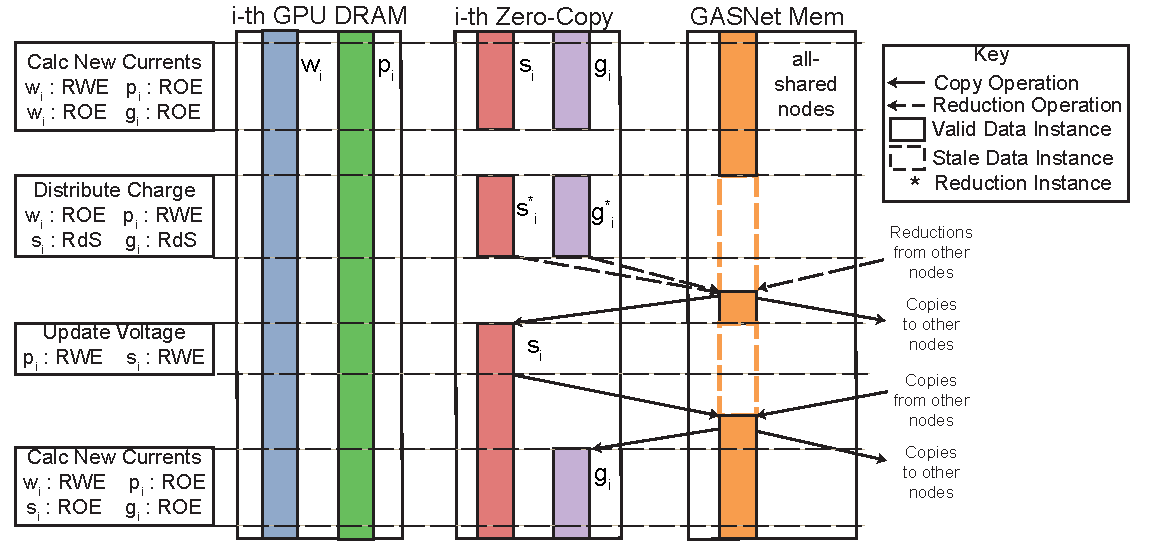
\includegraphics[scale=0.48]{figs/CircuitMem.pdf}
\caption{Tasks and data for the circuit simulation on a cluster of GPUs.}
\label{fig:gpumapping}
\end{figure}

Figure~\ref{fig:ckt_speed} shows the performance of the Legion circuit simulation relative
to a hand-coded single-GPU implementation written in CUDA.  The hand-coded implementation is
able to keep the entire simulation state in fast framebuffer memory.  Each line shows the scaling of
a particular problem size as the number of nodes is varied.  Our results demonstrate
excellent strong scaling, with speedups of 39.0X for the small problem on 48 GPUs and 
62.5X for the larger problem size on 96 GPUs.  The inset in the graph shows the relative
performance for small numbers of GPUs.  On a single GPU, our Legion implementation
is within 5\% of the performance of the hand-coded simulation.

Figure~\ref{fig:ckt_overhead} shows the fraction of the overall simulation time (summed over
all nodes) spent in the application kernels compared to the various pieces of the Legion
SOOP runtime.  As the node count increases, the non-communication overhead stays relatively constant.
As expected the communication overhead grow linearly with number of nodes.

\begin{figure}
\subfigure[Circuit simulation speed relative to single-GPU implementation.]
{
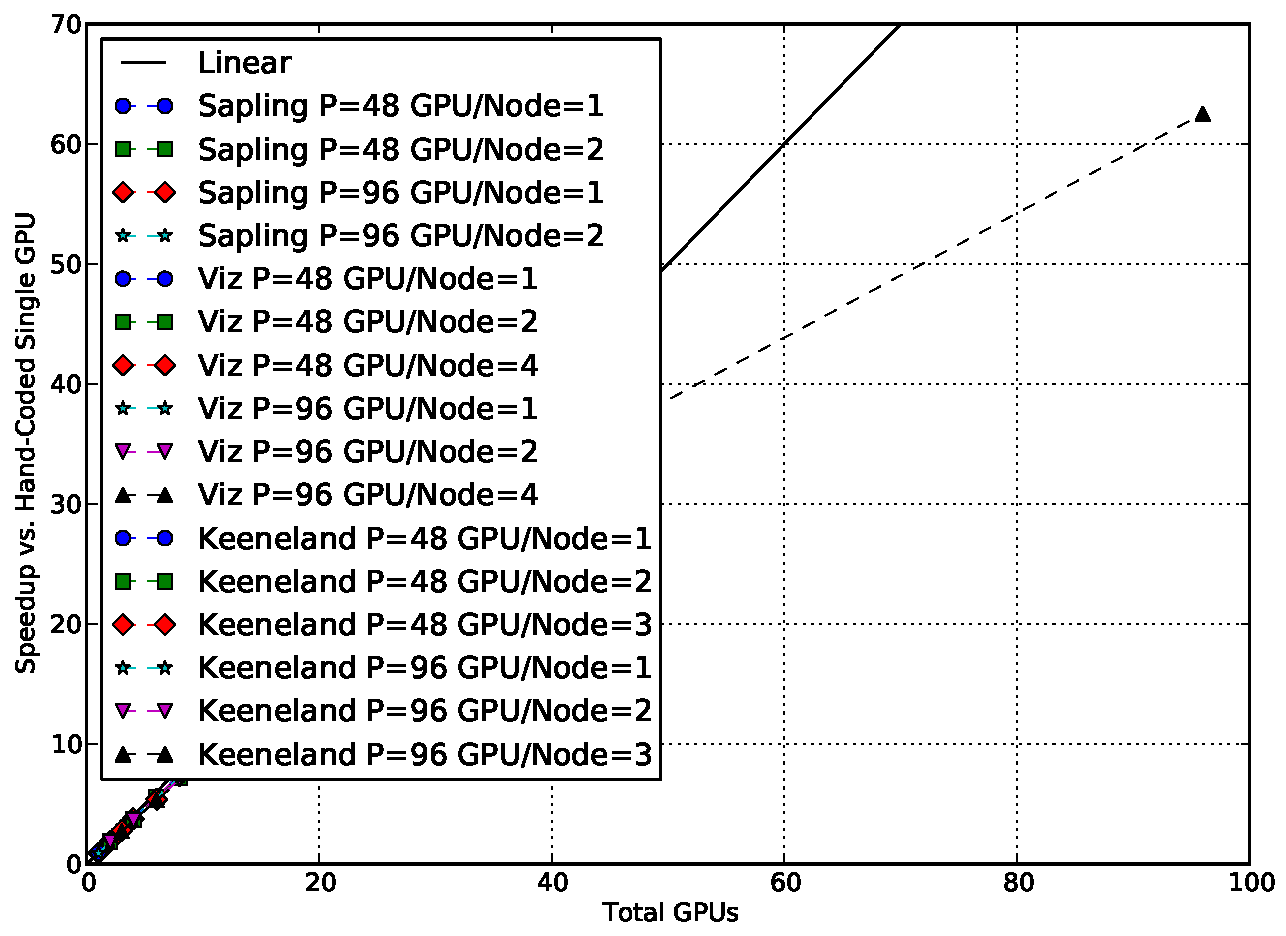
\includegraphics[scale=0.4]{figs/circuit_speedups.pdf}
\makebox[0pt][r]{
\raisebox{0.25 in}{
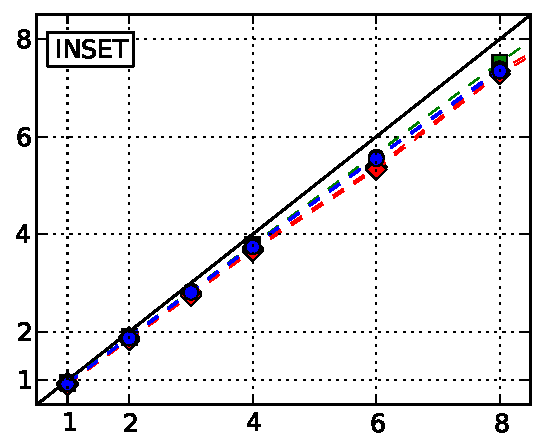
\includegraphics[scale=0.4]{figs/circuit_speedups_zoom.pdf}
}
}
\label{fig:ckt_speed}
}

\subfigure[Overhead of circuit simulation on Keeneland with 3 GPUs/node.]
{
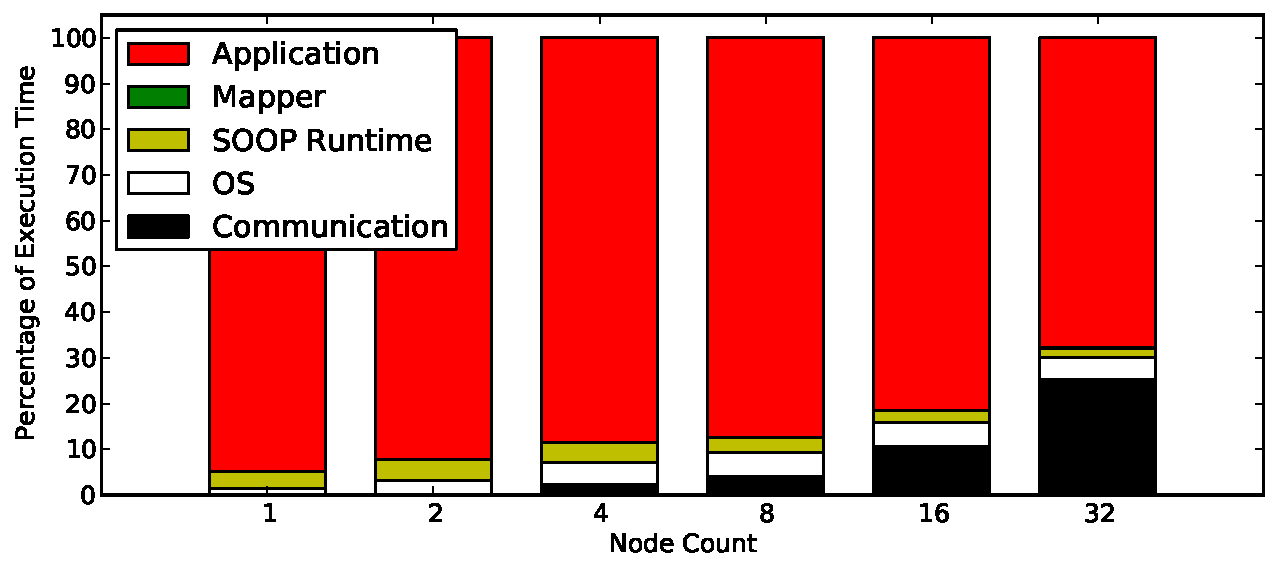
\includegraphics[scale=0.4]{figs/circuit_overhead.pdf}
\label{fig:ckt_overhead}
}
\vspace{-2mm}
\caption{Circuit simulation results.}
\vspace{-6mm}
\end{figure}

\subsection{Particle Simulation}
\label{subsec:exp_fluid}

Our second experiment is a port of the \emph{fluidanimate} benchmark
from the PARSEC benchmark suite\cite{bienia11benchmarking}, which does a
particle-based simulation of an incompressible fluid.  Each particle
interacts only with other nearby particles. The benchmark divides the
space in which the fluid can move into a three-dimensional array of
cells such that the range of interaction is limited to just the cells
adjacent (including diagonals) to the one a particle resides in.  The
application divides the array into {\em grids} and assigns each grid to
a thread.  Per-cell locking safely accesses particles in
cells that lie on the edge of a grid.  This fine-grained locking
scheme along with the assumption of a shared address space gives
good scaling in a multi-core processor, but rules out any attempt to run
beyond a single node.

To extend the scaling further, our port uses region partitioning to
divide the array into grids in a similar way, but avoids relying
on shared memory to handle interactions between grids.
Instead, the Legion version creates
explicit ghost copies of cells on grid boundaries and uses
those ghost cells to exchange information between the grids.

The particle simulation's mapper is very simple: it maps one grid's
tasks onto each processor and maps all that grid's regions (both
internal and ghost regions) into that processor's system memory.  The
exchange of ghost cell data between processors is handled by the
Legion runtime as a ghost cell region is alternately mapped to two
different memories.

Figure~\ref{fig:fluid_single} compares the performance of the Legion
implementation against the PARSEC version, using a relatively small
problem (300K particles on a 15x21x15 array of cells).  Speedups for
both the Legion and threaded PARSEC implementations are measured 
relative to PARSEC's serial version, which eliminates all locking
operations.  Between 1 and
4 threads, the PARSEC and Legion results are nearly indistinguishable,
indicating neither the Legion runtime nor the restructuring of the
implementation to allow multi-node scaling impose any significant
overhead.
%It's possible that the use of explicit ghost cells rather than fine-grained sharing of cache lines might be a net win.  
At 8 threads and above, performance begins to vary.  Both the Legion
and PARSEC versions on Viz flatten out as they over-subscribe the 12
physical cores.  On Sapling, which has HyperThreading enabled,
deviations from linear begin sooner as the operating system's
thread placement choices begin to matter.

To measure scaling beyond a single node, three different problem sizes
were run for each of the three systems (Figure~\ref{fig:fluid_multi}).
For the smallest problem (300K particles), we observe a 20\% speedup
from 1 to 2 nodes (16 threads total), but slow
down beyond that due to communication overhead---at 4 nodes there are
twice as many ghost cells as interior grid cells.  The larger problem
sizes (2.4M and 19M particles) do much better, with scaling of up to
5.4x when going from 1 node up to 16 because of a lower
communication-to-computation ratio.

%Although the particle simulation being performed is on a regular array of cells, it turns out that the
%distribution of particles amongst the cells is very irregular.  The simulation models gravity, which points in
%the -Y direction, so the particles are clustered mostly in the lower half of the cell array.  The PARSEC
%implementation works around this imbalance by only slicing the cell array through the X and Z axes, yielding
%grids that are uniformly populated, even if the number of boundary cells (for which locks must be used) is
%increased above the minimum. MORE TEXT NEEDED HERE

\begin{figure}
\subfigure[Single-node particle simulation speed.]
{
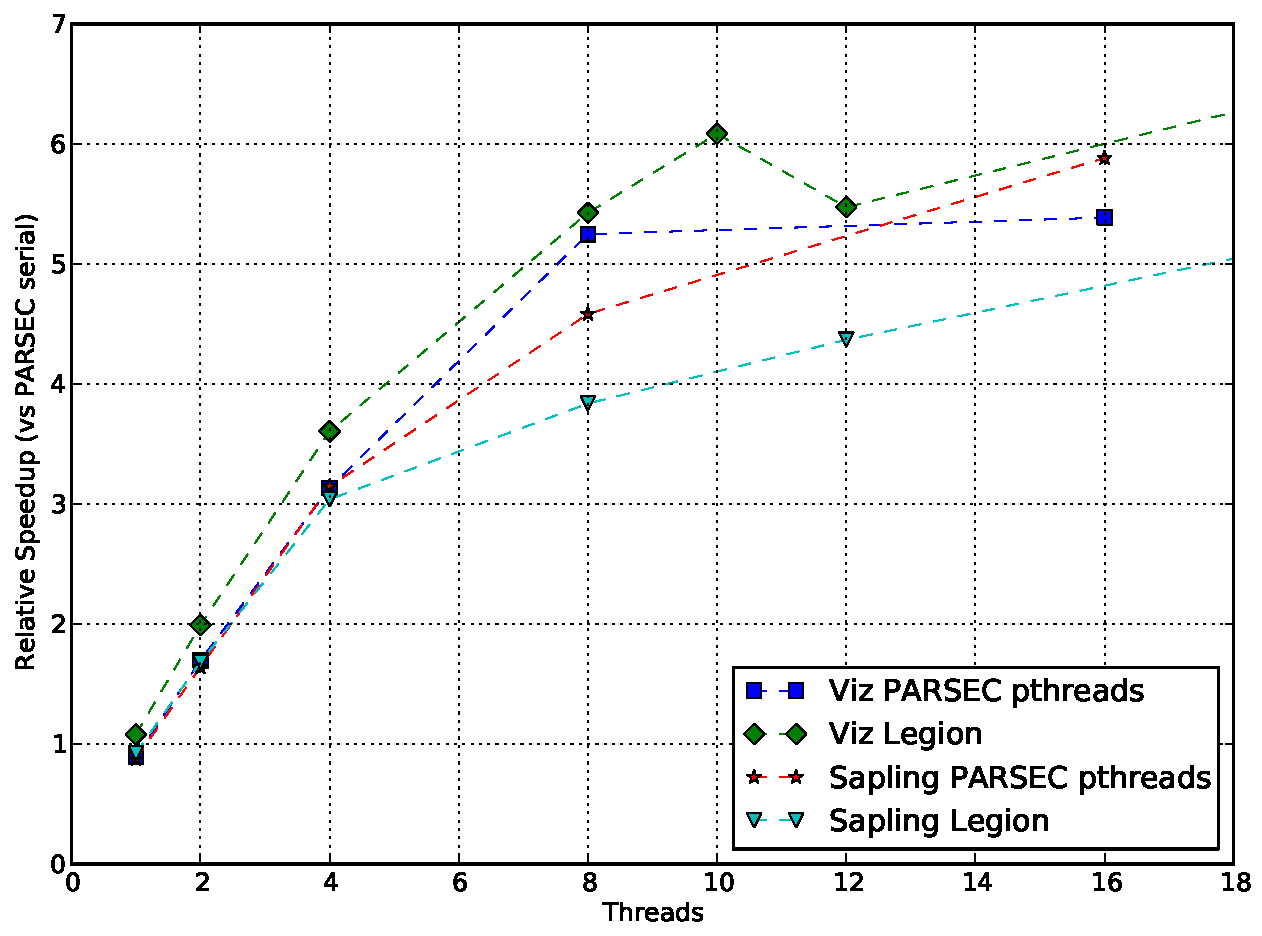
\includegraphics[scale=0.4]{figs/fluid_singlenode.pdf}
\label{fig:fluid_single}
}

\subfigure[Multi-node scaling.]
{
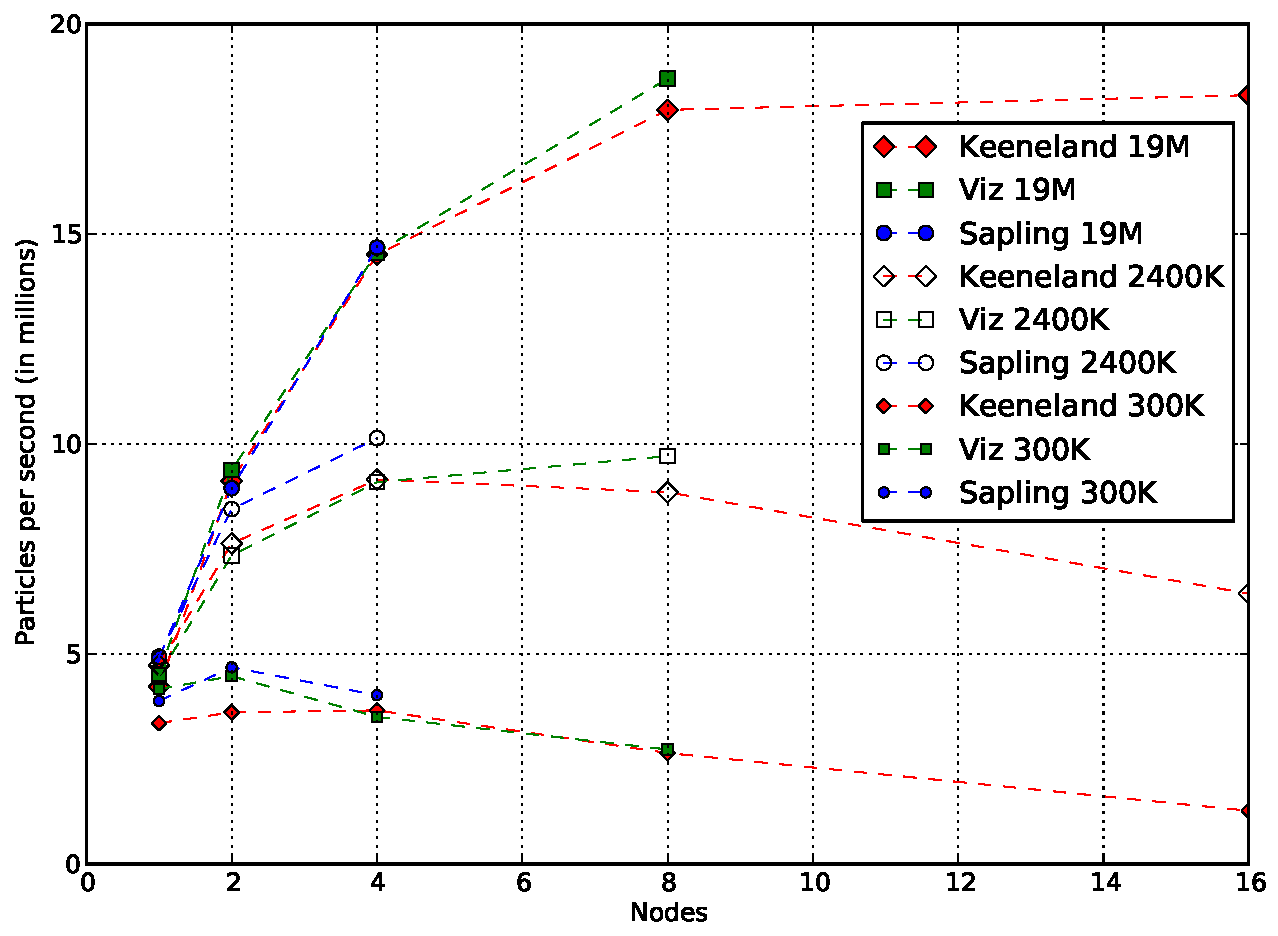
\includegraphics[scale=0.4]{figs/fluid_multinode.pdf}
\label{fig:fluid_multi}
}

%\subfigure[Effect of load-balanced partitioning.]
%{
%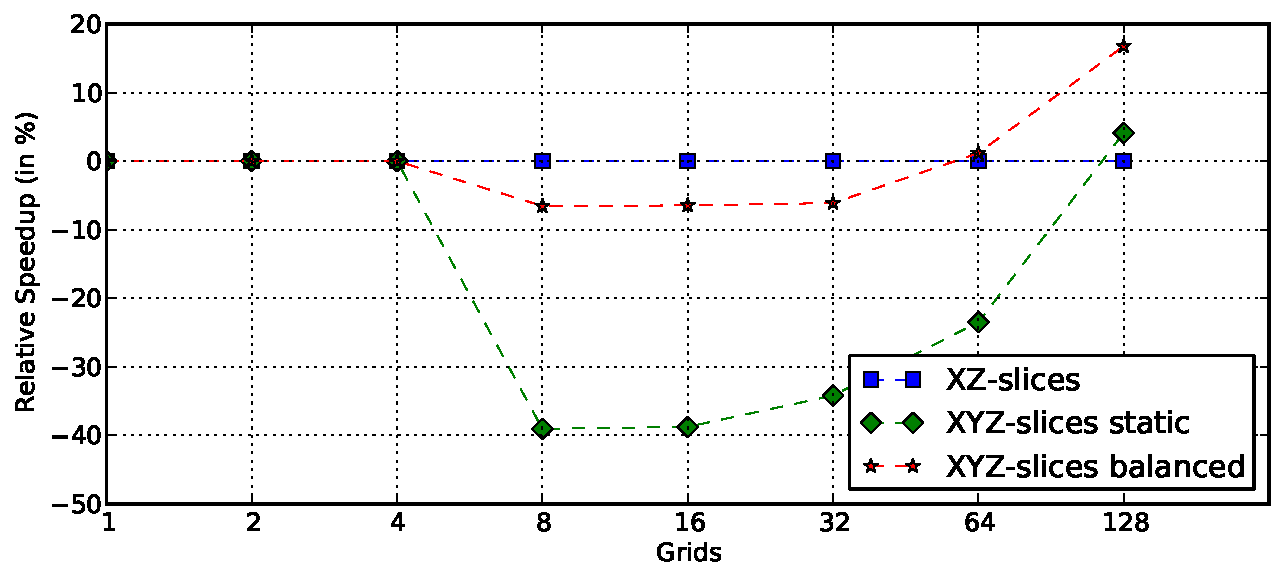
\includegraphics[scale=0.4]{figs/fluid_balance.pdf}
%\label{fig:fluid_balance}
%}
\vspace{-2mm}
\caption{Fluid simulation results.}
\vspace{-6mm}
\end{figure}

\subsection{Adaptive Mesh Refinement}
\label{subsec:exp_amr}
Our final application is based on the third heat equation example from
the Berkeley Labs BoxLib project \cite{BoxLib}.  This application is a
three-level adaptive-mesh-refinement (AMR) code that computes a first
order stencil on a 2D mesh of cells.  
%The simulation iterates for many time steps.  
Updating the simulation for one time step consists of
three phases.  In the first phase, the boundary cells around a box at
a refined level linearly interpolate their values from the nearby
cells at the next coarsest level.  The second phase performs the
stencil computation on each cell in every level.  In the third phase,
cells at a coarser level that have been refined are restricted to the
average of the cells that they physically contain at the next finest
level of refinement.

Achieving high-performance on this application is particularly
challenging for several reasons.  First, the application has a very
high communication-to-computation ratio which, for a fixed problem
size, begins as being memory bound and with increasing node count
becomes network bound as the perimeter-to-area ratio of cell grids
increases.  Second, when choosing how to partition cells into grids,
the programmer must consider the locality between cells within a
level as well as across levels.  For
cross-level cell dependences, mapping decisions must be made at
runtime as the location of refinements are dynamically determined.
Finally, this application has parallelism both
between tasks running at the same level and tasks running across
levels, leading to complicated input-dependent data dependences.

BoxLib's implementation partitions cells within a level 
into a number of grids based on the number of nodes in the
machine and distributes one grid from each level to each node.  This
optimizes for memory bandwidth and load balance, but does not 
exploit cross-level locality between grids from
different levels of refinement.  Furthermore, BoxLib does not block
grids into sub-grids to take advantage of intra-grid locality.

Our Legion implementation performs two optimizations that allow us to
outperform BoxLib.  First, for each level of
refinement we recursively partition the logical region of cells based
on the number of nodes in the machine and the sizes of the L2 and L3 caches.
%Legion allows us to describe locality for many levels of
%the memory hierarchy instead of just at the node-level.
Our second optimization takes advantage of the cross-level locality.
We wrote an application-specific mapper that dynamically discovers
relationships between grids at different levels of refinement.  The
mapper dynamically performs intersection tests between logical regions
containing grids of different refinement levels.  If the mapper
discovers overlaps between grids from different levels, the mapper
places them on the same node in the machine.  The
mapper memoizes the intersection tests to amortize their cost.  The
mapper also dynamically load balances by distributing unconstrained
grids from the coarsest level onto under-loaded nodes.

We compared our Legion implementation against BoxLib on three
different problem sizes with a fixed number of cells per level of
refinement, but with randomly chosen refinement locations.  BoxLib
also supports OpenMP and we took their best performance from using 1,
2, 4, or 8 threads per node.  Our Legion implementation always uses
one thread per node to illustrate that in this application locality is
significantly more important than parallelism.  

Figure~\ref{fig:amr_total} gives the results.
On just one node, blocking for caches using Legion achieves up to 2.6X
speedup over BoxLib.  As node count increases, the mapper's
ability to exploit cross-level locality further increases
the performance advantage to 5.4X by reducing the total
communication costs.

As the node count increases the AMR code becomes highly dependent on
interconnect performance.  BoxLib performs much better on Keeneland
than on Viz due to the better interconnect.  
At higher node counts BoxLib
begins to catch up (see Figure~\ref{fig:amr_keeneland})
because our intra-level ghost-cell exchange 
uses GASNet memory to exchange ghost cells, requiring a
linear increase in network traffic with the number of nodes.  BoxLib
uses direct node-to-node exchanges of ghost cells, similar to
our fluid application.  A future implementation of our AMR code will
employ a similar ghost cell exchange algorithm to improve scalability.

\begin{figure}
\subfigure[Sapling results.]
{
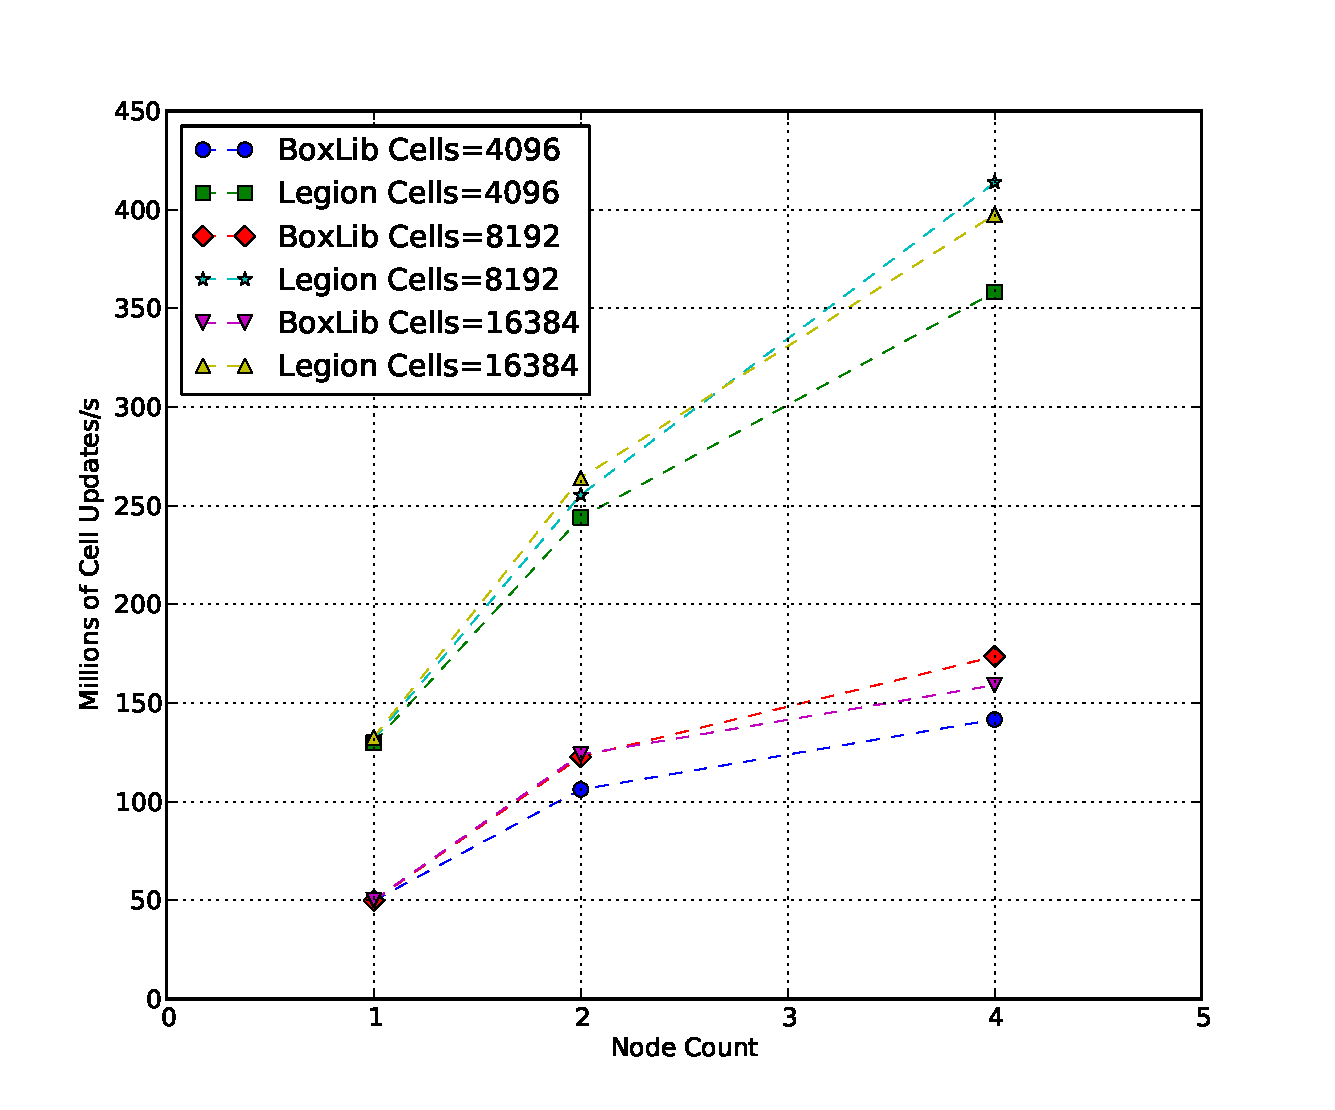
\includegraphics[scale=0.4]{figs/Sapling_amr.pdf}
\label{fig:amr_sapling}
}

\subfigure[Viz results.]
{
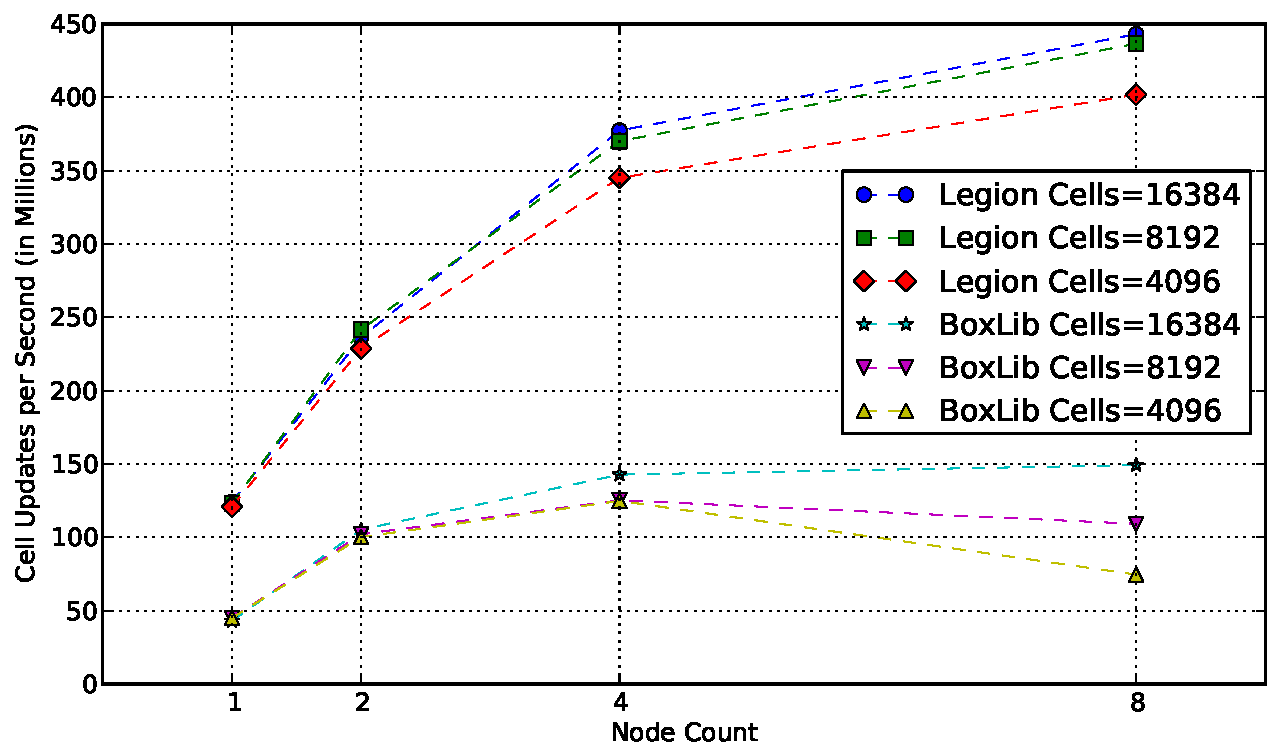
\includegraphics[scale=0.4]{figs/Viz_amr.pdf}
\label{fig:amr_viz}
}

\subfigure[Keeneland results.]
{
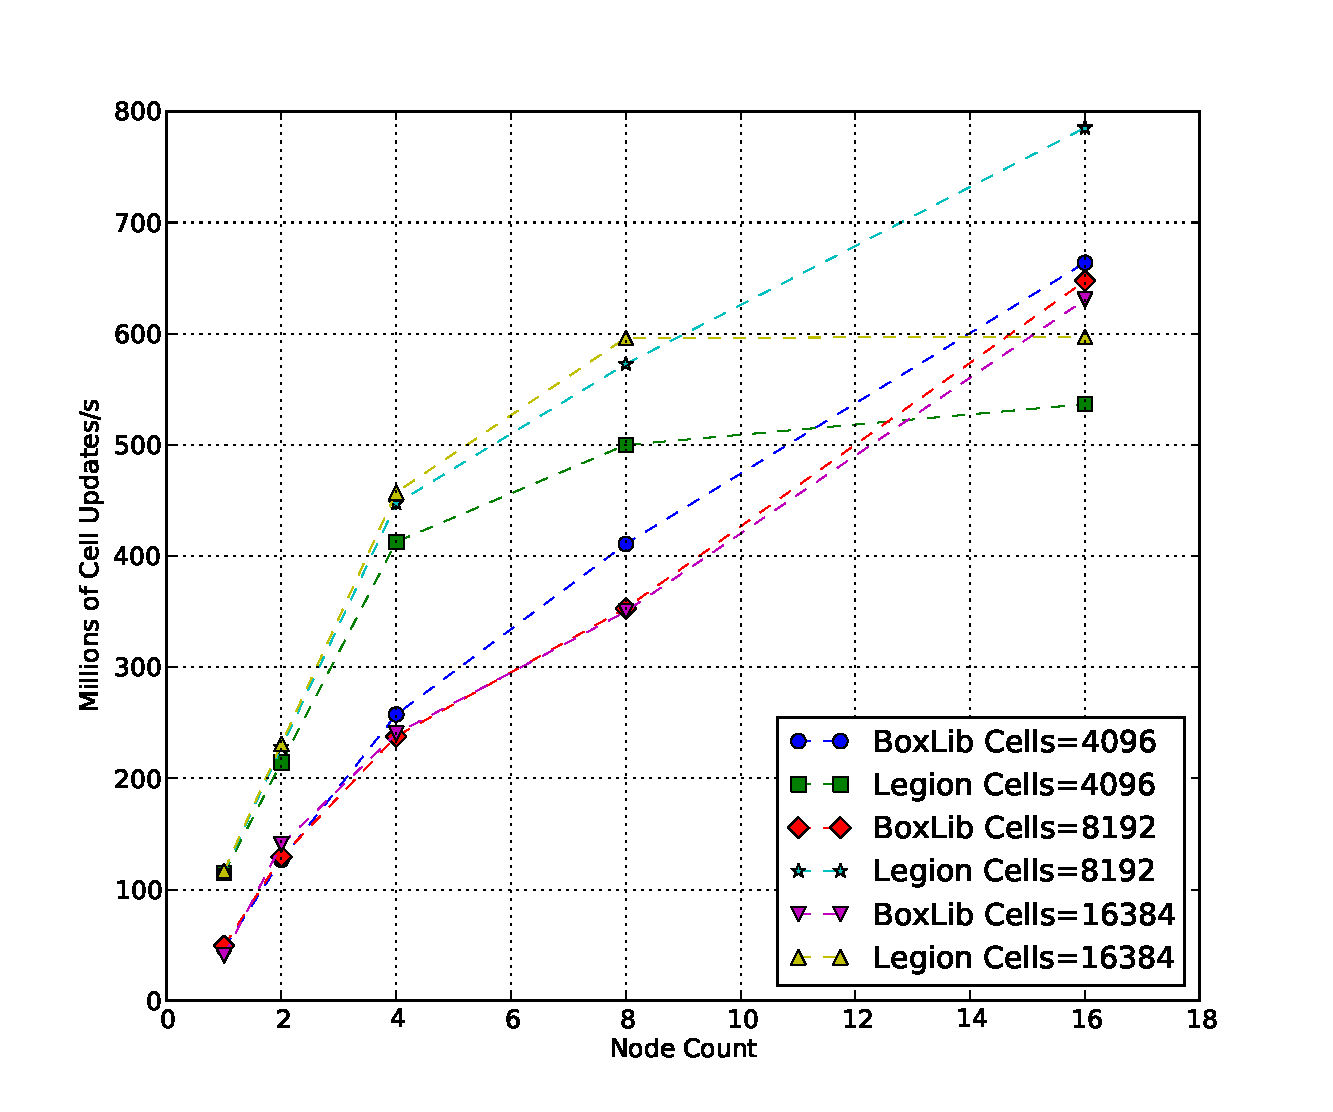
\includegraphics[scale=0.4]{figs/Keeneland_amr.pdf}
\label{fig:amr_keeneland}
}
\vspace{-2mm}
\caption{Throughput of adaptive mesh refinement code. \label{fig:amr_total}}
\vspace{-6mm}
\end{figure}


\section{Related Work}
\label{sec:related}
Legion is most directly related to Sequoia \cite{Fatahalian06}.  Sequoia is array-based, with
a limited repetoire of ways to partition arrays.  Sequoia is a static language with a single unified hierarchy
of tasks and data; Legion is more dynamic with separate task and region hierarchies.

Deterministic Parallel Java (DPJ) is the only other region-based parallel system of which we are
aware\cite{Bocchino09}.  While there are similarities in the permission system and we have
reused some DPJ notation, there are differences stemming from DPJ's static approach.
Regions in Legion are first-class and can be created, partitioned, packed, and unpacked 
dynamically, allowing programmers to compute data organization at runtime; like Sequoia, DPJ
partition schemes must be statically decided.  Legion allows 
programmers to create multiple partitions of the same region to give different 
views onto the same data, which is not possible in DPJ.  
%DPJ only supports the 
%equivalent to Legion's exclusive and atomic coherence modes \cite{Bocchino11} 
%while Legion provides safe execution even in simultaneous environments.  
There is also a difference in emphasis: DPJ requires shared memory, while Legion 
is designed for distributed heterogenous machines.

Chapel \cite{Chamberlain:Chapel} and X10 \cite{X1005} also provide some Legion-like facilities.
Chapel's domains and X10's places provide the programmer with a 
mechanism for expressing locality, similar to regions in Legion.  However, domains
and places are not used for independence analysis to discover parallelism.
In contrast, Jade uses annotations to describe
data disjointness,  and like Legion leverages the disjointness information
to discover parallelism, but lacks a region system to name and organize unbounded collections of objects \cite{Rinard98}.  

% Unclear to me what subtleties need to be pointed out here and explained
% to properly differentiate our work
Many efforts use static region systems for  memory management (e.g., \cite{Tofte94, Grossman02}).
Our system is more closely affiliated with dynamic region systems used for expressing locality for performance \cite{Gay01}.

%In addition to region languages with static type systems, there have been several
%dynamic region languages.  Cyclone uses both a static type system and dynamic
%region checks to enforce memory safety properties of C programs\cite{Grossman02}.
%Gay and Aiken introduced RC which reference counts regions dynamically and uses
%a static type system to reason about effeciently garbage collecting regions\cite{Gay01}.

There have been many type and effect systems for ownership types
\cite{Boyapati03} including ones that leverage nested regions for describing
relationships \cite{Clarke02,Cameron07}.  However, ownership type and effect systems
are primarily used for reasoning about determinism in object oriented languages and
don't capture the range of disjointness properties that can be specified in Legion.

Reasoning about disjoint heap data is the strong suit of separation logic \cite{Reynolds02}.  
Concurrent separation logic\cite{Brookes04} has been 
used both to parallelize sequential programs\cite{Raza09,Gotsman07} and to provide 
a mechanism for reasoning about independence\cite{Hayman06}.
While we have borrowed some separation logic notation, we ultimately chose to use a 
permissions system as our primary formalism because separation logic does not easily
support reasoning about the interleaving of operations to non-disjoint regions of memory.

% I'm also not sure how much detail to go into here.  DPJ spends a lot of time
% on these papers, but I'm not sure I understand all the details of these papers.
% DPJ also cites Lu06 here, but I'm not sure if we have to
%Type and effect systems have also been used to reason about regions.  FX presented
%the original type and effect system on regions \cite{Lucassen88}, but was restricted 
%to using a finite number of regions and was incapable of describing nested data
%structures.  

% Do we need to enumerate what these disjointness properties are (DPJ does)
%Type and effect systems have also been used in the context of parallelism to discover
%deadlocks and race conditions \cite{Boyapati02,Abadi06,Jacobs08}, but do not present 
%any mechanism for discovering parallelism.

%Still not sure what we want to put here.
% DPJ sites additional separation logic papers but they didn't seem very similar.
% Let me know if you think we should include them as well.





{
\small
\bibliography{bibliography}
}

\end{document}


